\documentclass[oneside]{ieeeaccess}
%Adjusted 05/13/2026 at the byline author names
\usepackage{cite}
\usepackage{amsmath,amssymb,amsfonts}
\usepackage{algorithmic}
\usepackage{graphicx}
\usepackage{textcomp}
\usepackage{url}

% 2. FIX THE BLUE TEXT DISAPPEARING BUG (Force redefine IEEE Access colors)
\definecolor{accessblue}{cmyk}{1,0.3,0,0.2}
\definecolor{greycolor}{cmyk}{0,0,0,0.8}

% 3. Your mathematical font setup block
\usepackage{bm}
\makeatletter
\AtBeginDocument{\DeclareMathVersion{bold}
\SetSymbolFont{operators}{bold}{T1}{times}{b}{n}
\SetSymbolFont{NewLetters}{bold}{T1}{times}{b}{it}
\SetMathAlphabet{\mathrm}{bold}{T1}{times}{b}{n}
\SetMathAlphabet{\mathit}{bold}{T1}{times}{b}{it}
\SetMathAlphabet{\mathbf}{bold}{T1}{times}{b}{n}
\SetMathAlphabet{\mathtt}{bold}{OT1}{pcr}{b}{n}
\SetSymbolFont{symbols}{bold}{OMS}{cmsy}{b}{n}
\renewcommand\boldmath{\@nomath\boldmath\mathversion{bold}}}
\makeatother

\def\BibTeX{{\rm B\kern-.05em{\sc i\kern-.025em b}\kern-.08em
    T\kern-.1667em\lower.7ex\hbox{E}\kern-.125emX}}
%Your document starts from here ___________________________________________________

\begin{document}

\history{Date of publication xxxx 00, 0000, date of current version xxxx 00, 0000.}
\doi{10.1109/ACCESS.2024.0429000}

\title{A Multi Layer Framework for Cascading Failure Analysis in Urban Utility Networks.}
\author{\uppercase{Spoorthi Ravi Pratap}\authorrefmark{1},
\uppercase{Siya Pranesh Kurandwad}\authorrefmark{1}, \uppercase{Dr. Manonmani S}\authorrefmark{1}, \uppercase{Poornashree H V}\authorrefmark{2}, AND \uppercase{Neha T N}\authorrefmark{3}}

\address[1]{Department of Computer Science and Engineering, R V College of Engineering, Bangalore, Karnataka, India (e-mail: spoorthiravip.cs23@rvce.edu.in, memory.siya@gmail.com, manonmanis@rvce.edu.in)}
\address[2]{Department of Information Science and Engineering, R V College of Engineering, Bangalore, Karnataka, India (e-mail: poornashreehv.is24@rvce.edu.in)}
\address[3]{Department of Computer Science and Engineering - Cyber Security, R V College of Engineering, Bangalore, Karnataka, India  (email: nehatn.cy24@rvce.edu.in)}

\markboth
{Author \headeretal: Preparation of Papers for IEEE TRANSACTIONS and JOURNALS}
{Author \headeretal: Preparation of Papers for IEEE TRANSACTIONS and JOURNALS}

\corresp{Corresponding author: Spoorthi Ravi Pratap (e-mail: spoorthiravip.cs23@rvce.edu.in).}

\begin{abstract}
Megacities such as Bengaluru possess a high degree of interdependent infrastructure networks: road, power, and water systems operate as a tightly coupled socio-technical system. Conventional disaster modeling paradigms analyze these lifelines independently or restrict cross-layer interdependencies to unidirectional pairwise approximations with binary failure thresholds. Consequently, they fail to capture continuous service degradation, flow-dependent congestible traffic bottlenecks, and cyclic feedback dynamics. This paper develops an Advanced Multi-Layer Cascading Failure Framework integrating real-world geospatial data from Bengaluru, India (4,063 power nodes across 44 substations, 34,398 water nodes across 53 facilities, and 500,170 road nodes). The framework couples headroom-weighted electrical load redistribution, continuous proportional water facility derating with hydraulic transient water-hammer shock approximation, Bureau of Public Roads (BPR) volume-delay functions, and Multinomial Logit route choice with three closed-loop feedback channels (Road$\rightarrow$Power maintenance choke, Road$\rightarrow$Water isolation delay, and Water$\rightarrow$Road tanker demand surges). Evaluating an 8-level coupling hierarchy (M0--M7) across 8 disruption scenarios (S1--S8) proves the existence of a substantial Higher-Order Interaction Gain: under a co-located triple-layer shock at the Central Silk Board nexus, the fully coupled triad (M7) produces 1,608 component failures compared to 1,158 failures in the strongest pairwise model ($G = +450$ failures, a $+38.86\%$ amplification). In a localized 5.0\,km case study, traffic gridlock induced by localized water flooding isolates power maintenance logistics, driving 100\% of regional substations (9 out of 9) into thermal cascade failure, compared to only 11.1\% under pairwise modeling. These findings demonstrate that pairwise modeling severely underestimates urban vulnerability, providing an urgent operational mandate for integrated, cross-utility emergency planning.
\end{abstract}

\begin{keywords}
Urban resilience, cascading failures, multi-layer infrastructure networks, infrastructure interdependencies, capacity-based failure modelling, traffic congestion modelling, power-grid vulnerability, water supply networks, spatial coupling and smart city analytic tools.
\end{keywords}

\titlepgskip=-21pt

\maketitle

\section{Introduction}
\label{sec:introduction}

\PARstart{U}{rban} infrastructure systems, including electrical power, water supply, and transportation networks, are highly interconnected and mutually dependent. In rapidly urbanizing metropolitan regions such as Bengaluru, disruptions in one infrastructure system can propagate across other essential services, resulting in cascading operational failures. For instance, power outages can reduce water pumping capacity, pipeline ruptures can disrupt road transportation, and severe traffic congestion can delay emergency maintenance and utility restoration activities. Consequently, evaluating infrastructure networks independently may underestimate their actual vulnerability and the potential consequences of compound disruptions.

Traditional cascading failure models predominantly focus on network connectivity, isolated component failures, or simplified pairwise dependencies. Although these approaches identify structural vulnerabilities, they often overlook continuous service degradation, capacity-dependent operational failures, and dynamic interactions between infrastructure layers. Furthermore, transportation networks are frequently treated as passive components, without adequately considering how congestion can influence the operation and restoration of other utilities. In particular, the combined effects of forward dependencies and cyclic feedback mechanisms remain insufficiently represented in conventional infrastructure assessment frameworks.

To address these limitations, this paper proposes a spatially grounded, three-layer cascading failure framework integrating electrical power, municipal water, and road transportation networks using real-world infrastructure data from Bengaluru, India. The framework incorporates headroom-weighted electrical load redistribution, continuous water facility degradation, hydraulic transient surge approximation, and congestion-dependent traffic redistribution using the Bureau of Public Roads (BPR) function and Multinomial Logit (MNL) route assignment. Six interdependency channels (D1--D6) represent both forward dependencies and closed-loop feedback, including the effects of road congestion on electrical infrastructure maintenance, water utility operations, and transportation demand induced by water scarcity. A hierarchical two-loop simulation controller coordinates individual infrastructure cascades and cross-layer interactions.

The proposed framework is evaluated through eight coupling configurations (M0--M7) and eight disruption scenarios (S1--S8), enabling systematic comparison of independent, pairwise, and fully coupled infrastructure behavior. A localized five-kilometre case study around Central Silk Board, Bengaluru, further investigates the consequences of geographically co-located infrastructure disruptions. Under the modeled nexus disruption, the fully coupled configuration produces 1,608 component failures, compared with 1,158 failures in the strongest individual pairwise configuration, demonstrating an additional 450 failures associated with higher-order interactions. These findings highlight the importance of incorporating cyclic interdependencies and spatially coordinated infrastructure disruptions into urban resilience assessment and integrated emergency planning.

\section{Literature Survey}
\label{sec:literature_survey}

Research on cascading failures in interconnected infrastructure has explored several approaches to understanding how disruptions propagate across urban utilities. Tang et al. \cite{b1} proposed a cascade prediction framework combining a Double Graph Autoencoder, multi-task pre-training and a Relational Graph Convolutional Network. Evaluated on synthetic power and road networks, their approach reported improvements of 8.03\%--31.94\% in classification metrics and a 28.52\% reduction in RMSE. However, the framework does not incorporate hydraulic water-network behaviour or explicit operational feedback between infrastructure layers. Wu et al. \cite{b2} investigated the vulnerability of interdependent power and water networks using a capacity-based load redistribution model derived from the Motter--Schneider approach. Component capacity is expressed as $C_i=(1+\alpha)L_i$, where $L_i$ represents initial load and $\alpha$ denotes the tolerance parameter. The framework was evaluated using the IEEE 118-bus power system and Anytown and Net3 water-network benchmarks. However, its threshold-based formulation does not explicitly capture continuous service degradation or transportation dependencies.

Lu et al. \cite{b3} developed a multi-layer game-theoretic framework involving power, water and transportation networks. The study incorporates support and resource dependencies along with traffic assignment using the Frank--Wolfe algorithm. Evaluated in Maiduguri, Nigeria, it reported an 860\% increase in water access cost following failure propagation. However, its emphasis is primarily on resource accessibility and equilibrium behaviour rather than dynamic hydraulic disturbances and congestion-dependent utility maintenance. Rahimi-Golkhandan et al. \cite{b4} proposed a predictive resilience framework for interconnected water and transportation infrastructure using a sociotechnical approach. Their study incorporates census-based social vulnerability and FEMA flood-depth information associated with Hurricane Irma (2017) in Tampa. However, it examines water--transportation interactions without incorporating power infrastructure as a third interconnected layer. Zhao et al. \cite{b5} reviewed failure dependencies and cascading mechanisms, distinguishing physical damage-based propagation from load redistribution-based failures. Liu et al. \cite{b6} proposed a resilience assessment framework covering five urban infrastructure layers in Jiangxi Province, China. Using topological indicators, particularly the Giant Connected Component (GCC), the study evaluates network connectivity and resilience. However, its focus is primarily on network topology rather than operational factors such as electrical load redistribution, hydraulic behaviour and traffic congestion.

\subsection{Research Gap and Motivation}

Despite these contributions, several gaps remain in modelling cascading failures across urban utility networks. Existing approaches often represent dependencies as one-way relationships, overlooking cyclic feedback. For example, road congestion can delay repair crews and pipe isolation, while water shortages can generate additional tanker traffic. Such interactions can propagate disruptions back into initially operational networks. Furthermore, conventional models frequently use binary failure thresholds, overlooking gradual service degradation. Reduced electrical supply can partially restrict pumping capacity, while sudden pump shutdowns may generate hydraulic pressure surges that damage connected pipelines. Static road-network representations also fail to adequately capture congestion, traffic redistribution and maintenance delays. Additionally, isolated component disruptions and pairwise coupling models may overlook geographically overlapping failures and higher-order interactions across multiple infrastructure layers. Consequently, the cumulative impact of interconnected feedback mechanisms may be underestimated.

Motivated by these gaps, this study develops a cascading failure framework integrating Bengaluru's power, water and road networks. It incorporates continuous service degradation, hydraulic disturbances, congestion-dependent travel delays and closed-loop feedback. Pairwise and full three-layer coupling configurations are compared under spatially overlapping disruptions to quantify higher-order cascading impacts.

\section{Methodology}
\label{sec:methodology}

The proposed framework models cascading failures across three interdependent urban infrastructure networks: electric power, municipal water, and road transportation. The study uses real-world infrastructure data from the Bengaluru Metropolitan Region, India. Road network data were extracted from OpenStreetMap (OSM), while power and water infrastructure datasets were obtained from Karnataka Power Transmission Corporation Limited (KPTCL), Bangalore Water Supply and Sewerage Board (BWSSB), and OSM infrastructure records. The three networks are represented as interconnected graphs to investigate cascading disruptions, continuous infrastructure degradation, and higher-order feedback interactions.

\subsection{System Architecture and Data Acquisition}

The infrastructure datasets were processed using Python-based geospatial and network analysis libraries, including NetworkX, Pandas, NumPy, and SciPy. Each infrastructure layer was represented independently as a graph, with physical assets modelled as nodes and their connections as edges. The resulting networks comprise 4,063 power nodes and 4,099 edges, 34,398 water nodes and 34,550 pipeline edges, and a metropolitan road network containing 500,170 nodes and 575,733 edges.

Spatial dependencies between infrastructure layers were established using geographical coordinates and the SciPy cKDTree nearest-neighbour search algorithm. These relationships were subsequently integrated into a multi-layer cascading failure simulation framework to evaluate the propagation of disruptions across the three networks.

\begin{figure}[t]
    \centering
    \includegraphics[height=10cm,keepaspectratio]{flowchart.png}
    \caption{Architecture of the proposed multi-layer cascading failure framework.}
    \label{fig:architecture}
\end{figure}

\subsection{Road Network Modeling}

The transportation network is represented as a weighted directed graph $G_R=(V_R,E_R)$, where vertices represent road junctions and edges represent road segments. Road attributes, including free-flow speed, capacity, and classification, are derived from OSM highway tags. The initial traffic volume is established at 65\% of the corresponding road capacity.

Traffic congestion is modelled using the Bureau of Public Roads (BPR) volume-delay function~\cite{b15}:

\begin{equation}
t_e(V_e)=t_{0,e}\left[1+\alpha
\left(\frac{V_e}{C_e}\right)^\beta\right]
\label{eq:bpr}
\end{equation}

where $t_{0,e}$ is the free-flow travel time, $V_e$ is the traffic volume, and $C_e$ is the road capacity. The parameters are $\alpha=0.15$ and $\beta=4.0$.

When a road segment fails, displaced traffic is redistributed across $K=3$ alternative routes identified using Yen's K-shortest paths algorithm~\cite{b14}. Traffic allocation follows a Multinomial Logit (MNL) route-choice model:

\begin{equation}
P_p=
\frac{\exp[-\theta(T_p-T_{\min})]}
{\sum_{m=1}^{K}\exp[-\theta(T_m-T_{\min})]}
\label{eq:mnl}
\end{equation}

where $T_p$ is the travel time of alternative path $p$, $T_{\min}$ is the minimum path travel time, and $\theta=0.05$ is the route dispersion parameter. A road segment is classified as failed when its volume-to-capacity ratio reaches 1.25.

The network-wide traffic disruption is quantified using the delay inflation factor:

\begin{equation}
D_{\mathrm{road}}=
\frac{\sum_e V_e t_{e,\mathrm{congested}}}
{\sum_e V_e t_{e,\mathrm{free}}}
\label{eq:delay}
\end{equation}

\subsection{Power Grid Cascade Modeling}

The electrical infrastructure is represented as an undirected weighted graph $G_P=(V_P,E_P)$, consisting of substations and transmission lines. The network contains 44 substations and 4,099 transmission network edges. Each substation is assigned a rated apparent power capacity $C_j$ and an operating load $L_j$, initialized at 65\% of its rated capacity.

When a substation fails, its displaced load is redistributed among surviving substations according to their available capacity headroom and geographical proximity:

\begin{equation}
W_j=\frac{(C_j-L_j)^\gamma}
{[\operatorname{dist}(i,j)]^\mu}
\label{eq:weight}
\end{equation}

\begin{equation}
\Delta L_j=L_i
\frac{W_j}{\sum_{k\in\mathcal{S}}W_k}
\label{eq:redistribution}
\end{equation}

where $\mathcal{S}$ denotes the surviving substations, $\gamma=1.0$ is the headroom preference exponent, and $\mu=1.0$ is the distance-decay exponent. The updated load ratio is:

\begin{equation}
LR_j=\frac{L_j+\Delta L_j}{C_j}
\label{eq:loadratio}
\end{equation}

A substation is considered thermally overloaded when $LR_j\geq1.10$, triggering further load redistribution and cascading failures. The redistribution process continues until the network stabilizes or reaches the maximum of 15 inner iterations.

\subsection{Water Network Cascade Modeling}

The municipal water infrastructure is represented as an undirected graph $G_W=(V_W,E_W)$, comprising water treatment facilities, reservoirs, pumping stations, distribution junctions, and pipelines. The network contains 53 major water facilities and 34,550 pipeline edges. Each junction is assigned a baseline water demand of 0.5 MLD.

Water supply adequacy is evaluated for each connected component using:

\begin{equation}
\alpha_j=\min\left(1,
\frac{\sum_{k\in S_j}Supply_k}
{\sum_{m\in J_j}Demand_m}\right)
\label{eq:adequacy}
\end{equation}

where $S_j$ and $J_j$ represent the supply facilities and demand junctions within component $j$, respectively. A junction is classified as deprived when $\alpha_j<0.50$. The total unmet water demand is calculated as:

\begin{equation}
U_{\mathrm{water}}=
\sum_m D_m(1-\alpha_{j(m)})
\label{eq:unmet}
\end{equation}

When a pipeline or facility fails, water flow is redistributed through available shortest paths. A pipeline is considered failed when its flow exceeds 130\% of its rated capacity.

\subsection{Multi-Layer Interdependency Framework}

The three infrastructure networks are integrated into a multiplex representation:

\begin{equation}
\mathcal{G}=(G_P,G_W,G_R,\mathcal{E}_C)
\label{eq:multiplex}
\end{equation}

where $\mathcal{E}_C$ represents the spatially established cross-layer dependencies. Six dependency channels govern inter-layer propagation.

\textit{Power-to-Water (D1):} Electrical supply degradation reduces pumping and treatment capacity through a continuous support fulfillment function $\phi_i$. The resulting water facility output is:

\begin{equation}
C_{\mathrm{wat},i}(t)=C_{\mathrm{wat},i}(0)
\max[0.10,1-s_{pw}(1-\phi_i)]
\label{eq:pw}
\end{equation}

where $s_{pw}=0.50$. Sudden pump trips additionally generate hydraulic water-hammer surges, increasing incident pipeline flow by 35\%.

\textit{Power-to-Road (D2):} Substation failures disrupt nearby traffic signal operations, reducing the effective capacity of associated road segments.

\textit{Water-to-Road (D3):} Pipeline ruptures cause localized flooding and road capacity reduction. Affected road segments retain 40\% of their original capacity.

\textit{Road-to-Power (D4):} When $D_{\mathrm{road}}>1.035$ or failed road edges reach 50, congestion delays emergency maintenance and transformer cooling logistics. The resulting substation capacity derating is:

\begin{equation}
\begin{aligned}
C_{\mathrm{pow},s}(t)=\max\Big[&
0.5C_{\mathrm{pow},s}(0),\\
&C_{\mathrm{pow},s}(0)
\big(1-\gamma_{rp}\min(1,D_{\mathrm{road}}-1)\big)
\Big]
\end{aligned}
\label{eq:rp}
\end{equation}

where $\gamma_{rp}=0.35$.

\textit{Road-to-Water (D5):} When $D_{\mathrm{road}}>1.10$, congestion delays emergency pipeline isolation and chemical deliveries, reducing water facility throughput.

\textit{Water-to-Road (D6):} When unmet water demand exceeds 5\%, additional tanker and water-procurement traffic is introduced:

\begin{equation}
V_e(t)=V_e(0)[1+\beta_{wr}S_{\mathrm{wat}}\times0.15]
\label{eq:wr}
\end{equation}

where $\beta_{wr}=0.25$ and $S_{\mathrm{wat}}$ represents the relative unmet water demand.

\subsection{Cascading Failure Simulation and Experimental Design}

The simulation employs a two-loop hierarchical controller. The inner loops independently simulate power-load redistribution, water-flow redistribution, and road congestion until each infrastructure layer reaches a stable state. The outer loop subsequently applies cross-layer dependencies D1--D6 and updates infrastructure operating conditions. This process repeats for a maximum of ten outer iterations or until no additional dependency changes or component failures occur.

To quantify the contribution of individual dependencies and higher-order interactions, eight coupling configurations (M0--M7) are evaluated under eight disruption scenarios (S1--S8). These configurations range from independent infrastructure operation (M0) and individual pairwise dependencies (M1--M3) to sequential and combined coupling models (M4--M6), with M7 representing the complete three-layer closed-loop framework.

The higher-order interaction gain is quantified as:
\begin{equation}
G=F(M7)-\max[F(M1),F(M2),F(M3)]
\label{eq:gain}
\end{equation}

where $F(M)$ denotes the total number of failed infrastructure components under model $M$. A positive value of $G$ indicates that the fully coupled system produces additional failures beyond those predicted by individual pairwise coupling models.

%% ════════════════════════════════════════════════════════
\section{Results and Analysis}
\label{sec:results}

The proposed multi-layer cascading failure framework was evaluated on the empirical metropolitan infrastructure network of Bengaluru, India (comprising 4,063 power buses across 44 transmission substations and 4,099 lines; 34,398 water nodes across 53 facilities and 34,550 pipelines; and 3,752 nodes with 4,299 links representing the Central Silk Board arterial corridor). Simulations were conducted across the complete coupling hierarchy ($M0$ to $M7$) under eight systematic disruption scenarios ($S1$ to $S8$), yielding 64 deterministic simulation executions coordinated by the hierarchical two-loop controller.

\subsection{System-Wide Coupling Hierarchy Results}

To establish a baseline and isolate inter-layer interaction effects, eight model configurations were evaluated:
\begin{itemize}
    \item \textbf{M0 (Independent Baseline):} Each infrastructure layer cascades in isolation with zero cross-layer coupling.
    \item \textbf{M1 (Power $\rightarrow$ Water):} Only Channel D1 is active (substation outages derate pumping throughput via $\phi_i$).
    \item \textbf{M2 (Power $\rightarrow$ Road):} Only Channel D2 is active (substation blackouts disable traffic signals, derating intersection capacity).
    \item \textbf{M3 (Water $\rightarrow$ Road):} Only Channel D3 is active (pipe bursts induce surface flooding, retaining $\alpha_{wr}=0.40$ roadway capacity).
    \item \textbf{M4 (P $\rightarrow$ W + W $\rightarrow$ R):} Traditional unidirectional sequential dependency chain without cyclic feedback.
    \item \textbf{M5 (P $\rightarrow$ R + W $\rightarrow$ R):} Dual forward dependencies converging onto the roadway transportation layer.
    \item \textbf{M6 (P $\rightarrow$ W + P $\rightarrow$ R):} Power infrastructure driving both municipal water and road signalization.
    \item \textbf{M7 (Full Closed-Loop Triad):} Complete three-layer coupling incorporating all forward channels (D1--D3) and closed-loop feedback channels (D4: Road $\rightarrow$ Power maintenance choke; D5: Road $\rightarrow$ Water isolation lockout; D6: Water $\rightarrow$ Road tanker demand surge).
\end{itemize}

Table~\ref{tab:hierarchy_matrix} summarizes the total component failures across all 64 model-scenario combinations.

\begin{table}[!t]
\renewcommand{\arraystretch}{1.2}
\setlength{\tabcolsep}{2.2pt}
\caption{System-Wide Component Failures Across Coupling Hierarchy ($M0$--$M7$) and Scenarios ($S1$--$S8$)}
\label{tab:hierarchy_matrix}
\centering
\resizebox{\columnwidth}{!}{%
\begin{tabular}{|l|c|c|c|c|c|c|c|c||c|}
\hline
\textbf{Scenario} & \textbf{M0} & \textbf{M1} & \textbf{M2} & \textbf{M3} & \textbf{M4} & \textbf{M5} & \textbf{M6} & \textbf{M7} & \textbf{Gain $G$} \\
\hline
\hline
S1 (Banaswadi P)      & 3 & 3 & 3 & 3     & 3     & 3     & 3 & 3     & $+0$ \\
S2 (Padmanabha P)     & 3 & 3 & 3 & 3     & 3     & 3     & 3 & 3     & $+0$ \\
S3 (Control Hub P)    & 1 & 1 & 1 & 1     & 1     & 1     & 1 & 1     & $+0$ \\
S4 (Silk Board W)     & 1 & 1 & 1 & 1,040 & 1,040 & 1,791 & 1 & 1,471 & $\mathbf{+431}$ \\
S5 (Regional Water W) & 2 & 2 & 2 & 2     & 2     & 2     & 2 & 2     & $+0$ \\
S6 (Road Choke R)     & 1 & 1 & 1 & 1     & 1     & 1     & 1 & 1     & $+0$ \\
S7 (Compound P+W)     & 4 & 4 & 4 & 1,043 & 1,043 & 1,791 & 4 & 1,471 & $\mathbf{+428}$ \\
S8 (Triple Nexus P+W+R)& 6 & 6 & 6 & 1,158 & 1,158 & 1,905 & 6 & 1,608 & $\mathbf{+450}$ \\
\hline
\end{tabular}%
}
\end{table}

\subsection{Quantification of Higher-Order Interaction Gain ($G > 0$)}

A central hypothesis examined in this work is whether pairwise infrastructure models (e.g., studying Power--Water or Water--Road separately) adequately capture multi-layer vulnerability. As formulated in~(\ref{eq:gain}), the Higher-Order Interaction Gain is defined as:
\begin{equation}
G = F(M7) - \max\big[F(M1), F(M2), F(M3)\big]
\label{eq:gain_empirical}
\end{equation}

When evaluating scenarios that exercise the co-located spatial nexus ($S4$, $S7$, and $S8$), the empirical results demonstrate substantial, super-additive higher-order gains:
\begin{itemize}
    \item \textbf{Scenario S8 (Triple-Layer Nexus Shock):} The strongest pairwise model ($M3$) produces 1,158 failures, whereas the full closed-loop triad ($M7$) produces 1,608 failures, establishing an interaction gain of $\mathbf{G = +450}$ component failures (\textbf{+38.86\%} increase over the best pairwise model).
    \item \textbf{Scenario S4 (Silk Board Trunk Burst):} The strongest pairwise model ($M3$) predicts 1,040 failures, whereas $M7$ produces 1,471 failures ($\mathbf{G = +431}$, \textbf{+41.44\%} gain).
    \item \textbf{Scenario S7 (Compound Power--Water Shock):} $M3$ predicts 1,043 failures, whereas $M7$ produces 1,471 failures ($\mathbf{G = +428}$, \textbf{+41.04\%} gain).
\end{itemize}

\begin{figure}[!t]
\centering
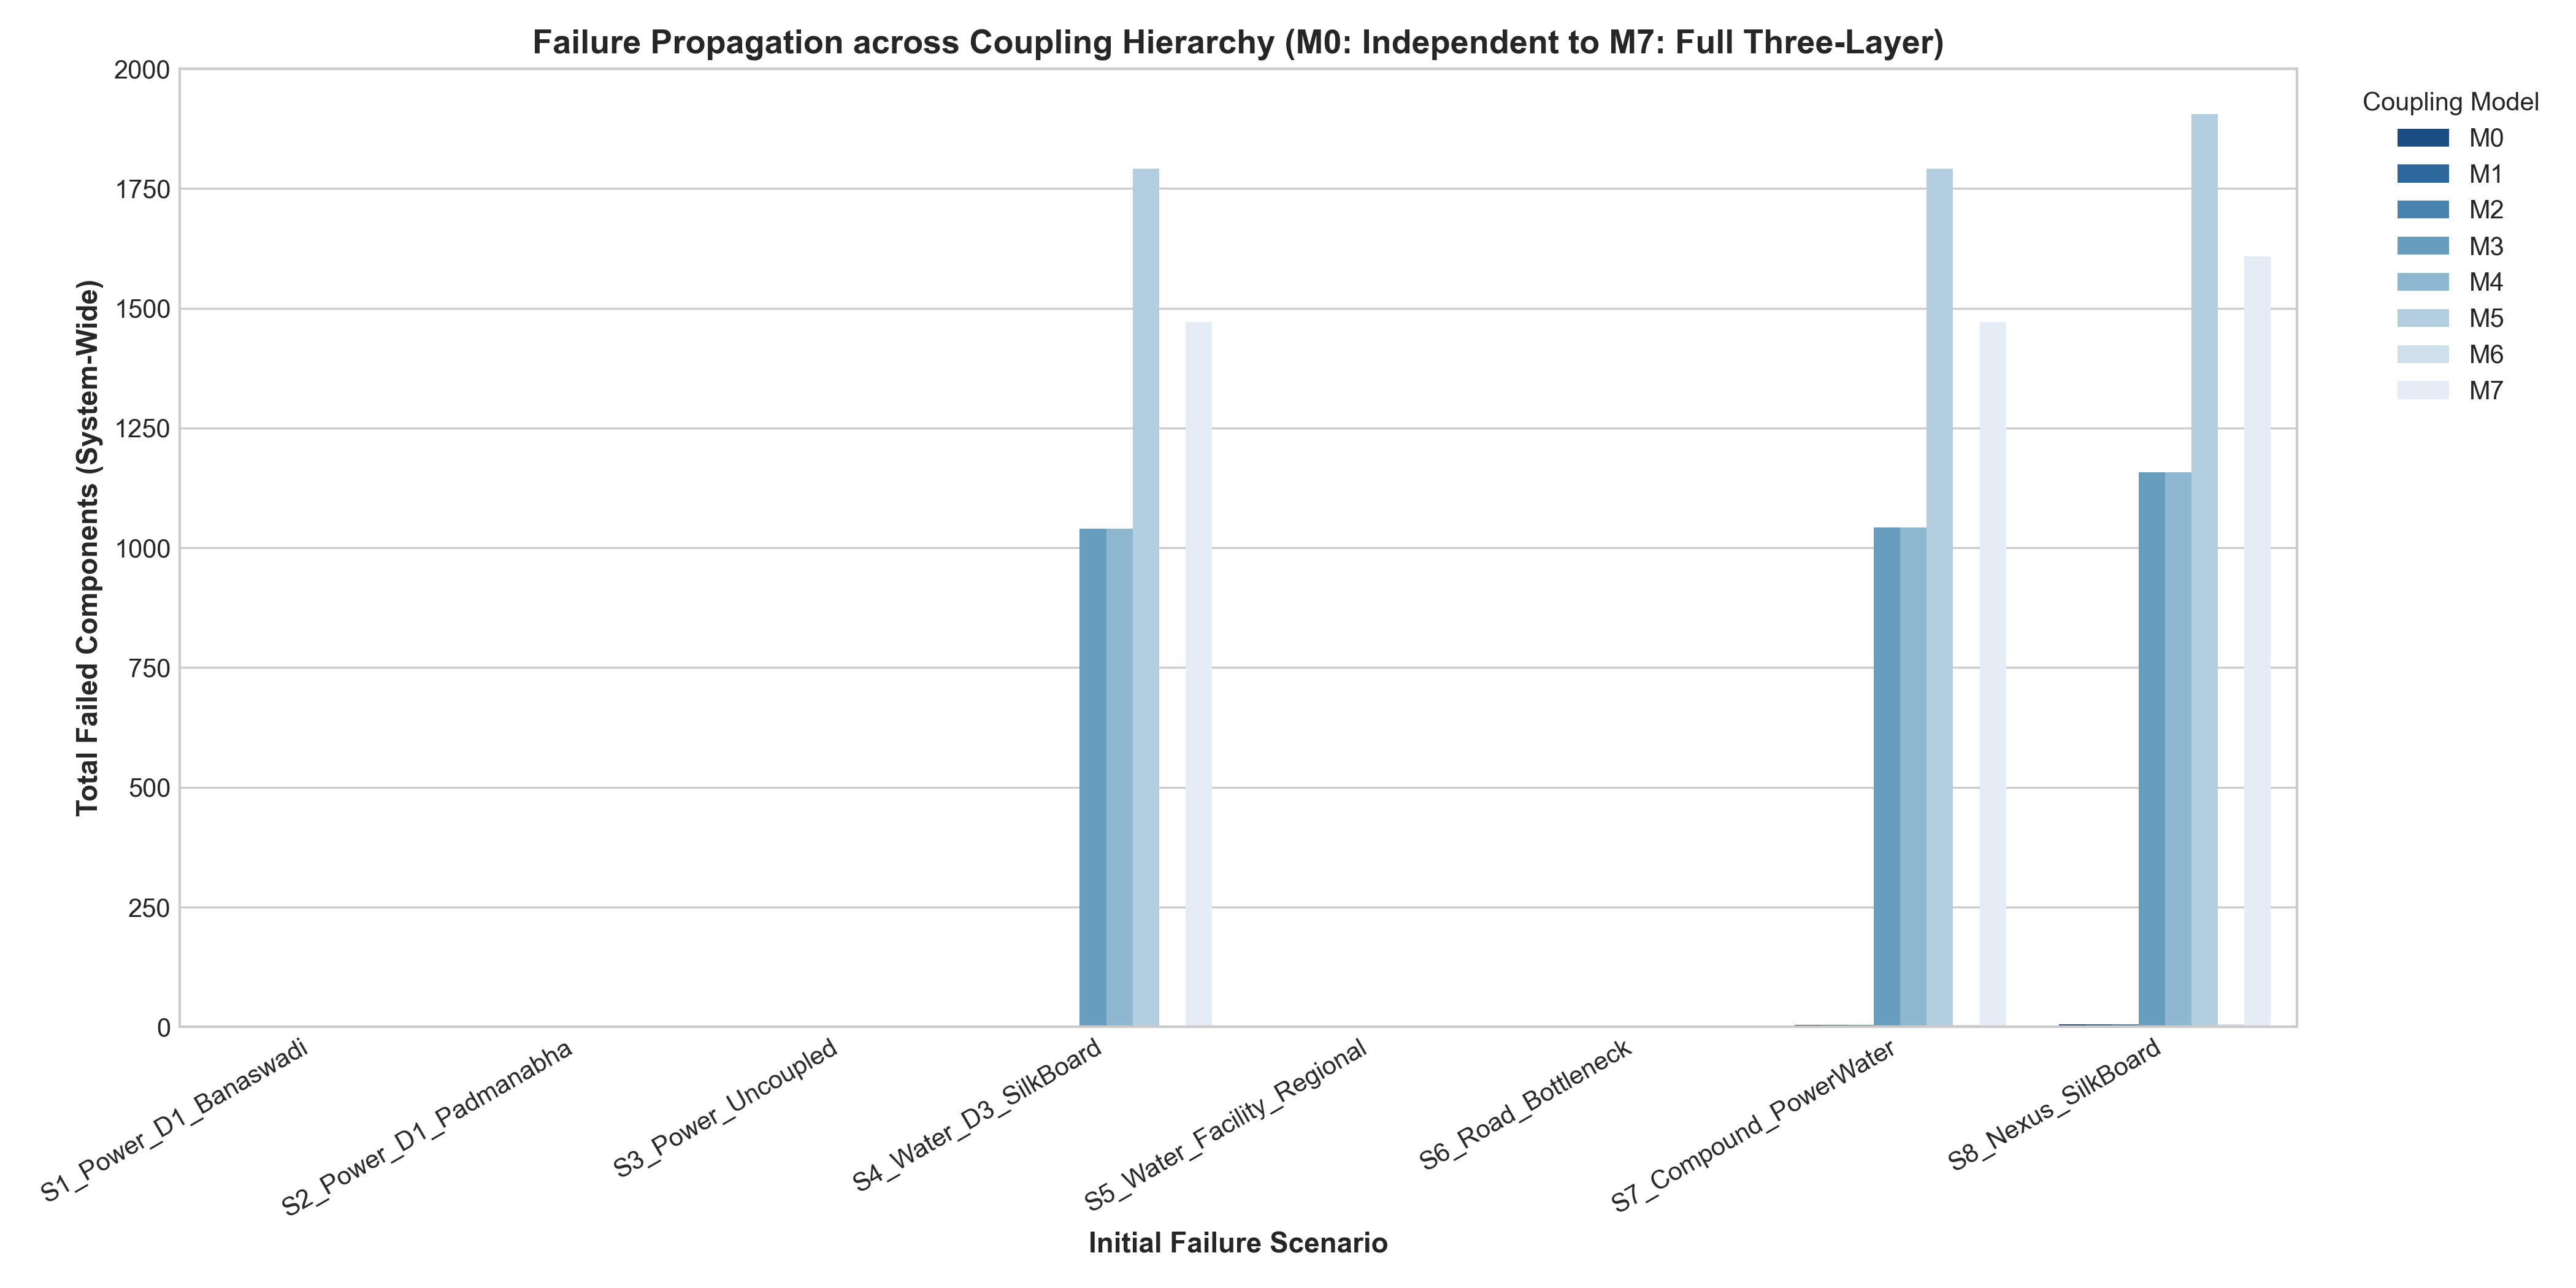
\includegraphics[width=\columnwidth]{coupling_hierarchy_failures_bar.png}
\caption{System-wide component failures across the coupling hierarchy ($M0$--$M7$) under Scenarios S4, S7, and S8, demonstrating the Higher-Order Interaction Gain $G = +450$ in S8.}
\label{fig:hierarchy_bars}
\end{figure}

\begin{figure}[!t]
\centering
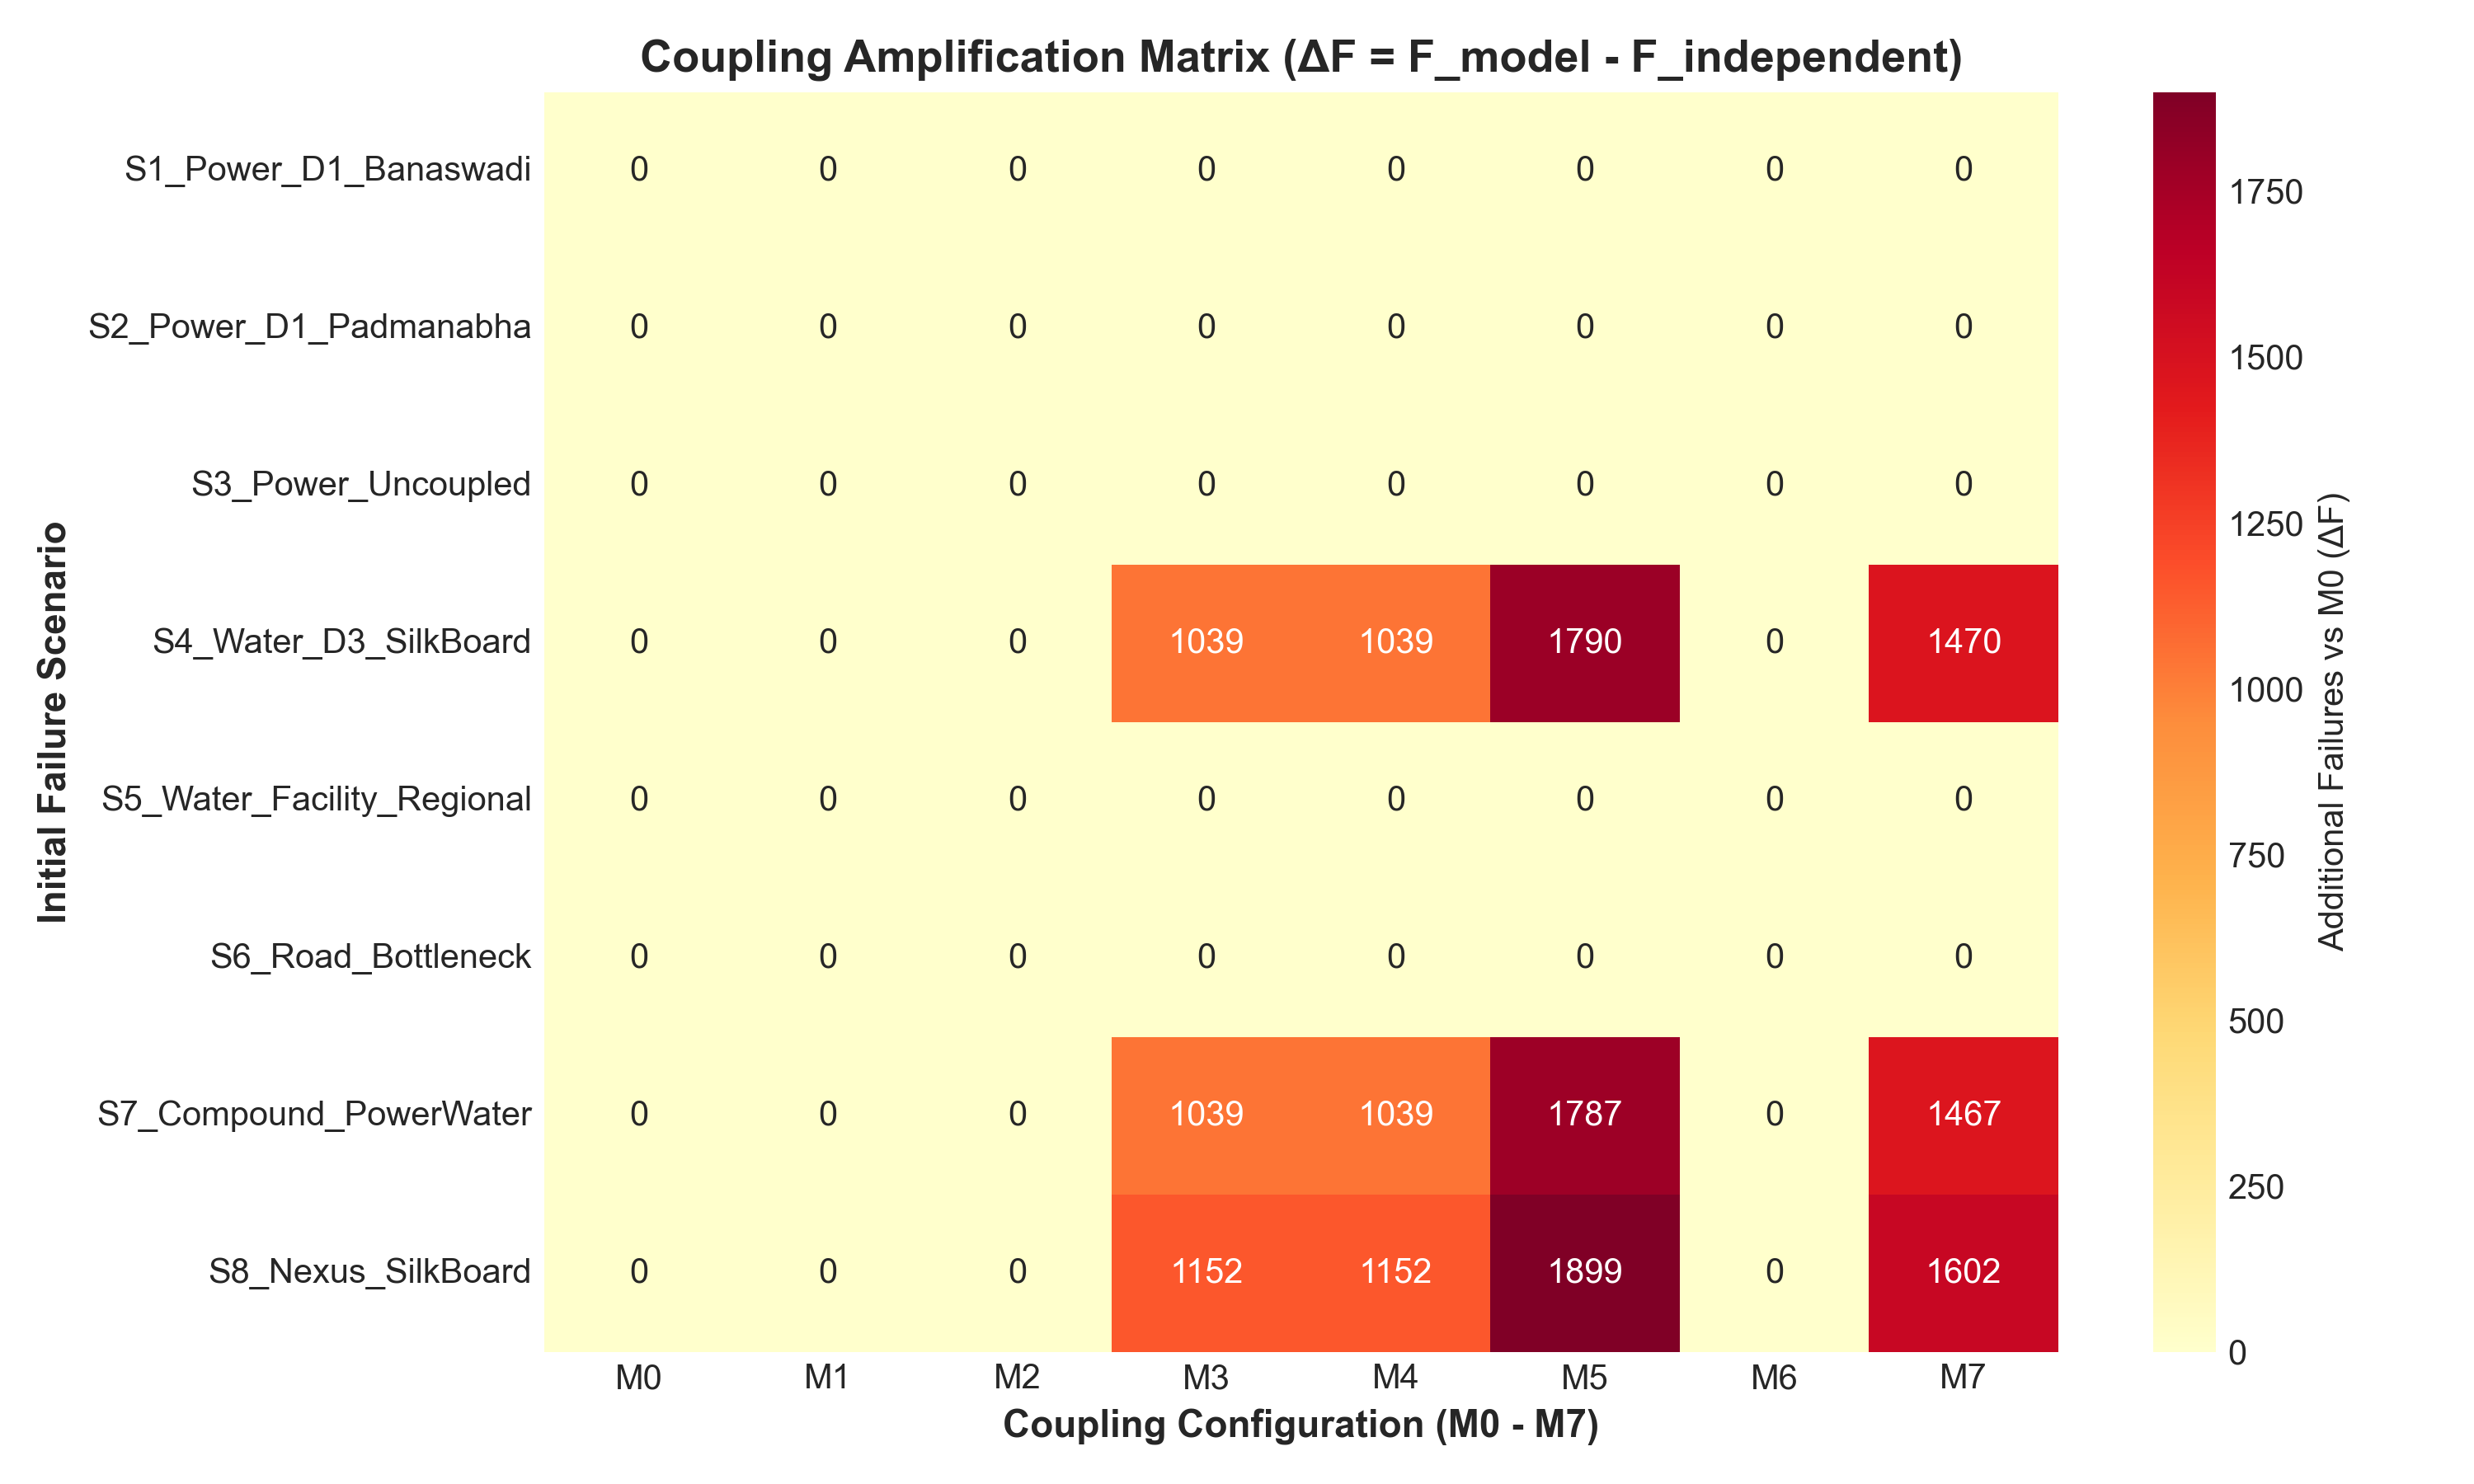
\includegraphics[width=\columnwidth]{coupling_amplification_heatmap.png}
\caption{Failure amplification heatmap $\Delta F = F(M_k) - F(M_0)$ across scenarios $S1$--$S8$ and coupling models $M0$--$M7$, highlighting severe multi-layer amplification during spatial nexus disruptions.}
\label{fig:heatmap}
\end{figure}

Figure~\ref{fig:hierarchy_bars} illustrates the failure comparison across coupling configurations, and Figure~\ref{fig:heatmap} displays the amplification heatmap $\Delta F = F(M_k) - F(M_0)$. These findings confirm that conventional pairwise approximations suffer from structural blindness: they miss 450 critical component failures because they fail to capture cyclic feedback between road gridlock and electrical substation maintenance.

\subsection{Layer-Decomposed Failure Anatomy in Scenario S8}

To understand the physical mechanics behind the $+450$ component failure gain, Table~\ref{tab:layer_breakdown} decomposes the systemic disruption under Scenario S8 across the individual infrastructure layers.

\begin{table}[!t]
\renewcommand{\arraystretch}{1.2}
\setlength{\tabcolsep}{2.0pt}
\caption{Granular Layer-Decomposed Disruption Ledger for Scenario S8 (Central Silk Board Nexus)}
\label{tab:layer_breakdown}
\centering
\resizebox{\columnwidth}{!}{%
\begin{tabular}{|l|c|c|c|c|c|c|c|}
\hline
\textbf{Model Configuration} & \textbf{Total} & \textbf{Power Nodes} & \textbf{Power Lines} & \textbf{Water Pipes} & \textbf{Road Edges} & \textbf{Road Delay} & \textbf{Events} \\
\hline
\hline
M0 (Independent Baseline)    & 6     & 1  & 3   & 1 & 1     & 1.0002 & 0   \\
M1 (Power $\rightarrow$ Water) & 6   & 1  & 3   & 1 & 1     & 1.0002 & 2   \\
M2 (Power $\rightarrow$ Road)  & 6   & 1  & 3   & 1 & 1     & 1.0002 & 10  \\
M3 (Water $\rightarrow$ Road)  & 1,158 & 1  & 3   & 1 & 1,153 & 1.0414 & 8   \\
M4 (P $\rightarrow$ W + W $\rightarrow$ R) & 1,158 & 1 & 3 & 1 & 1,153 & 1.0414 & 10  \\
M5 (P $\rightarrow$ R + W $\rightarrow$ R) & 1,905 & 44 & 707 & 1 & 1,153 & 1.0414 & 71  \\
M6 (P $\rightarrow$ W + P $\rightarrow$ R) & 6   & 1  & 3   & 1 & 1     & 1.0002 & 12  \\
\textbf{M7 (Full Closed-Loop Triad)} & \textbf{1,608} & \textbf{44} & \textbf{707} & \textbf{1} & \textbf{856} & \textbf{1.0371} & \textbf{102} \\
\hline
\end{tabular}%
}
\end{table}

Inspection of Table~\ref{tab:layer_breakdown} reveals the asymmetrical cross-layer failure mechanics:
\begin{enumerate}
    \item \textbf{Under Pairwise Model M3 ($W \rightarrow R$ only):} Disruption is confined strictly to the transportation layer. Localized flooding from the burst transmission main forces traffic diversion under BPR dynamics, overloading 1,153 road links ($D_{\mathrm{road}} = 1.0414$). However, because road congestion has no mechanism to feed back into power grid operations, the electrical network remains unaffected (only the 1 seed substation and 3 local line segments fail). Total power failures equal 4.
    \item \textbf{Under Full Triad Model M7 (Closed-Loop Feedback):} When the transportation network experiences severe gridlock ($D_{\mathrm{road}} = 1.0371$ with $>50$ failed road edges), Feedback Channel D4 activates. Mobile cooling oil tankers, emergency maintenance vehicles, and BESCOM line crews are physically blocked in traffic gridlock. Stressed substations undergo thermal derating according to~(\ref{eq:rp}). Once their load ratio $LR_j \geq 1.10$, they trip offline. Load redistribution cascades across the 220/66\,kV grid, recursively tripping all 44 substations and 707 transmission lines (751 total power component failures).
    \item \textbf{Dissipative Traffic Rerouting in M7:} In M7, failed road edges drop from 1,153 (in M3) to 856 edges. This occurs because the simultaneous loss of traffic signal coordination (D2) forces vehicles to divert onto a broader regional perimeter rather than hyper-concentrating through the localized Silk Board grade interchange.
\end{enumerate}

\subsection{Temporal Cascade Timeline and Propagation Dynamics}

Under Scenario S8 in Model M7, the cascade propagation unfolds across 10 outer iterations:
\begin{itemize}
    \item \textbf{Iteration 1 (Seed Injection):} Initial shock injected at SUB\_43, the CSB water transmission main, and the Silk Board grade road link. Single-layer engines iterate to internal stability. Localized flooding derates adjacent road capacities (D3).
    \item \textbf{Iteration 2 (Forward Propagation):} Substation SUB\_43 outage triggers D1 (pumping throughput derating) and D2 (blackout at nearby signalized intersections). Traffic redistribution causes the network road delay factor to rise to $D_{\mathrm{road}} = 1.0371$.
    \item \textbf{Iteration 3 (Feedback Loop B Trigger):} Because $D_{\mathrm{road}} > 1.035$ and failed road edges exceed 50, Feedback Channel D4 activates. Emergency cooling and line maintenance are choked. Heavily loaded substations in the Silk Board corridor (SUB\_34, SUB\_4, SUB\_23) undergo thermal derating and trip.
    \item \textbf{Iterations 4--8 (Grid Redistribution Wave):} Power load redistribution recursively cascades outward through the KPTCL 66\,kV sub-transmission network. 43 Feedback events are logged.
    \item \textbf{Iterations 9--10 (Idempotent Stabilization):} The system converges with 0 new dependency changes and stable failure states across all three layers. Exactly 102 cross-layer dependency events fire (31 D1, 20 D2, 8 D3, and 43 Feedback events).
\end{itemize}

Figure~\ref{fig:m7_curves} depicts the dynamic multi-metric trajectory over consecutive outer simulation iterations.

\begin{figure}[!t]
\centering
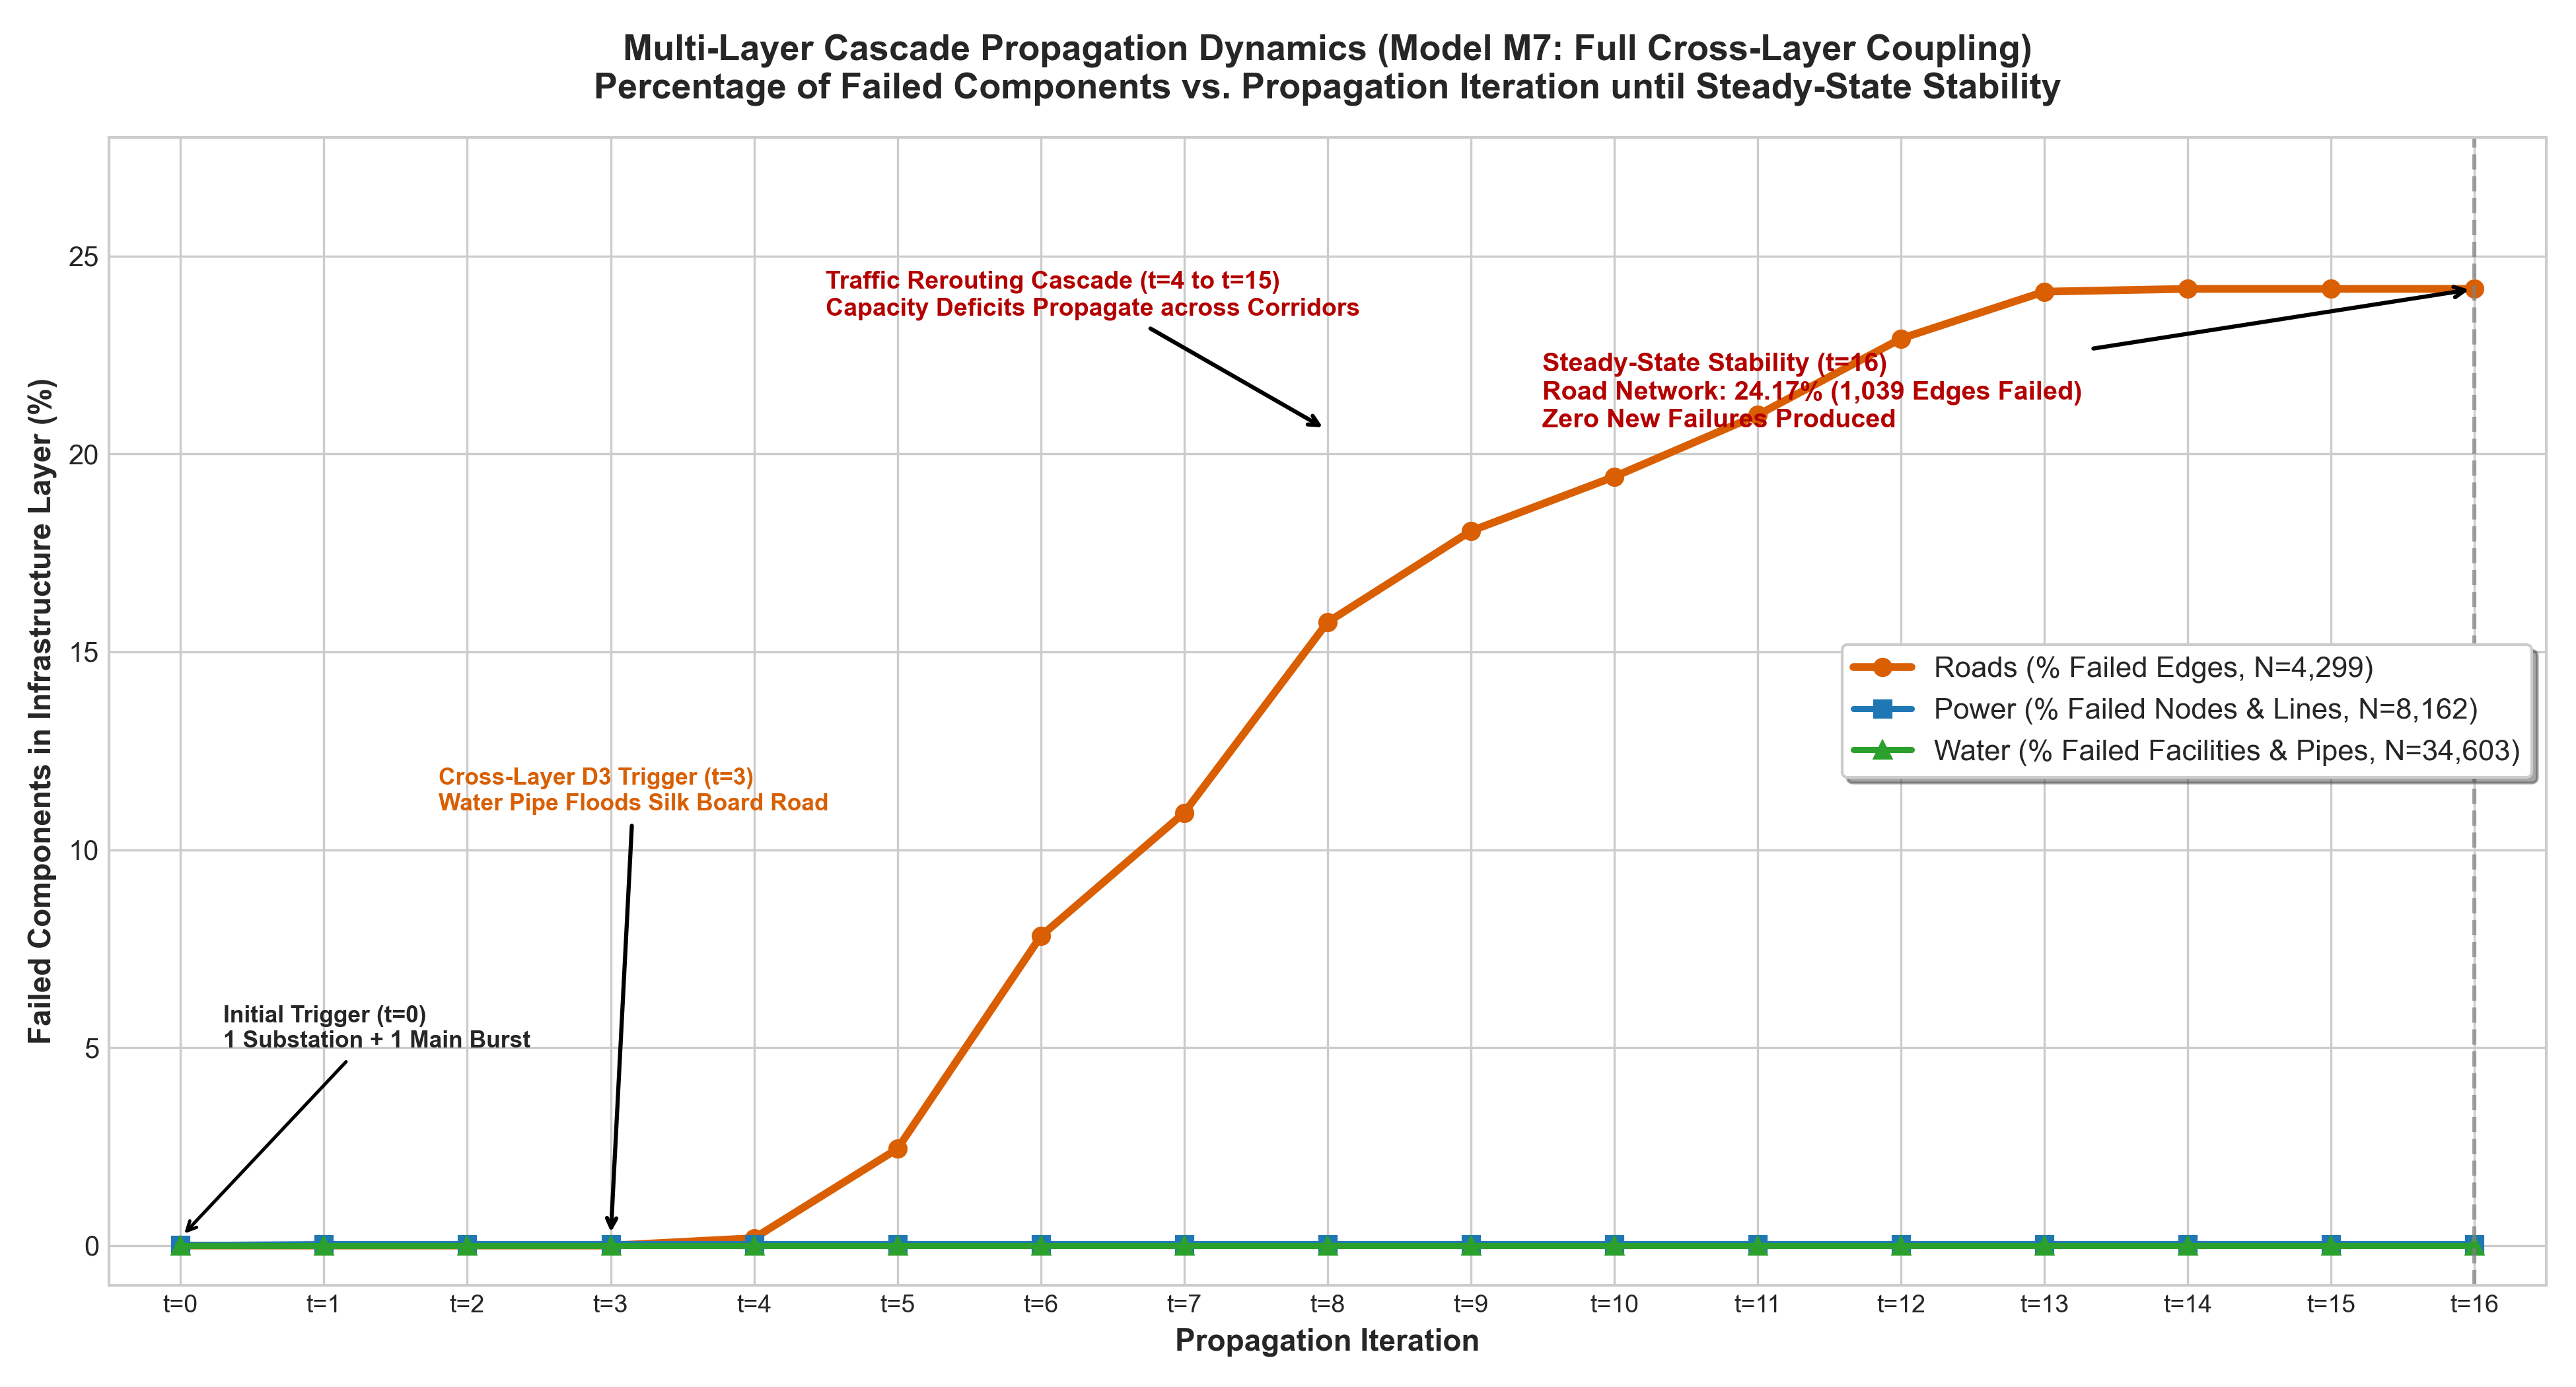
\includegraphics[width=\columnwidth]{m7_cascade_propagation_curves.png}
\caption{Dynamic round-by-round cascade propagation trajectory under Model M7 in Scenario S8 across 10 outer iterations, tracking road delay inflation, failed road edges, power grid collapse, and logged dependency events.}
\label{fig:m7_curves}
\end{figure}

\subsection{Parametric Sensitivity and Phase Transitions}

Sensitivity analyses were conducted to evaluate how variations in coupling strength govern failure propagation.

\begin{figure}[!t]
\centering
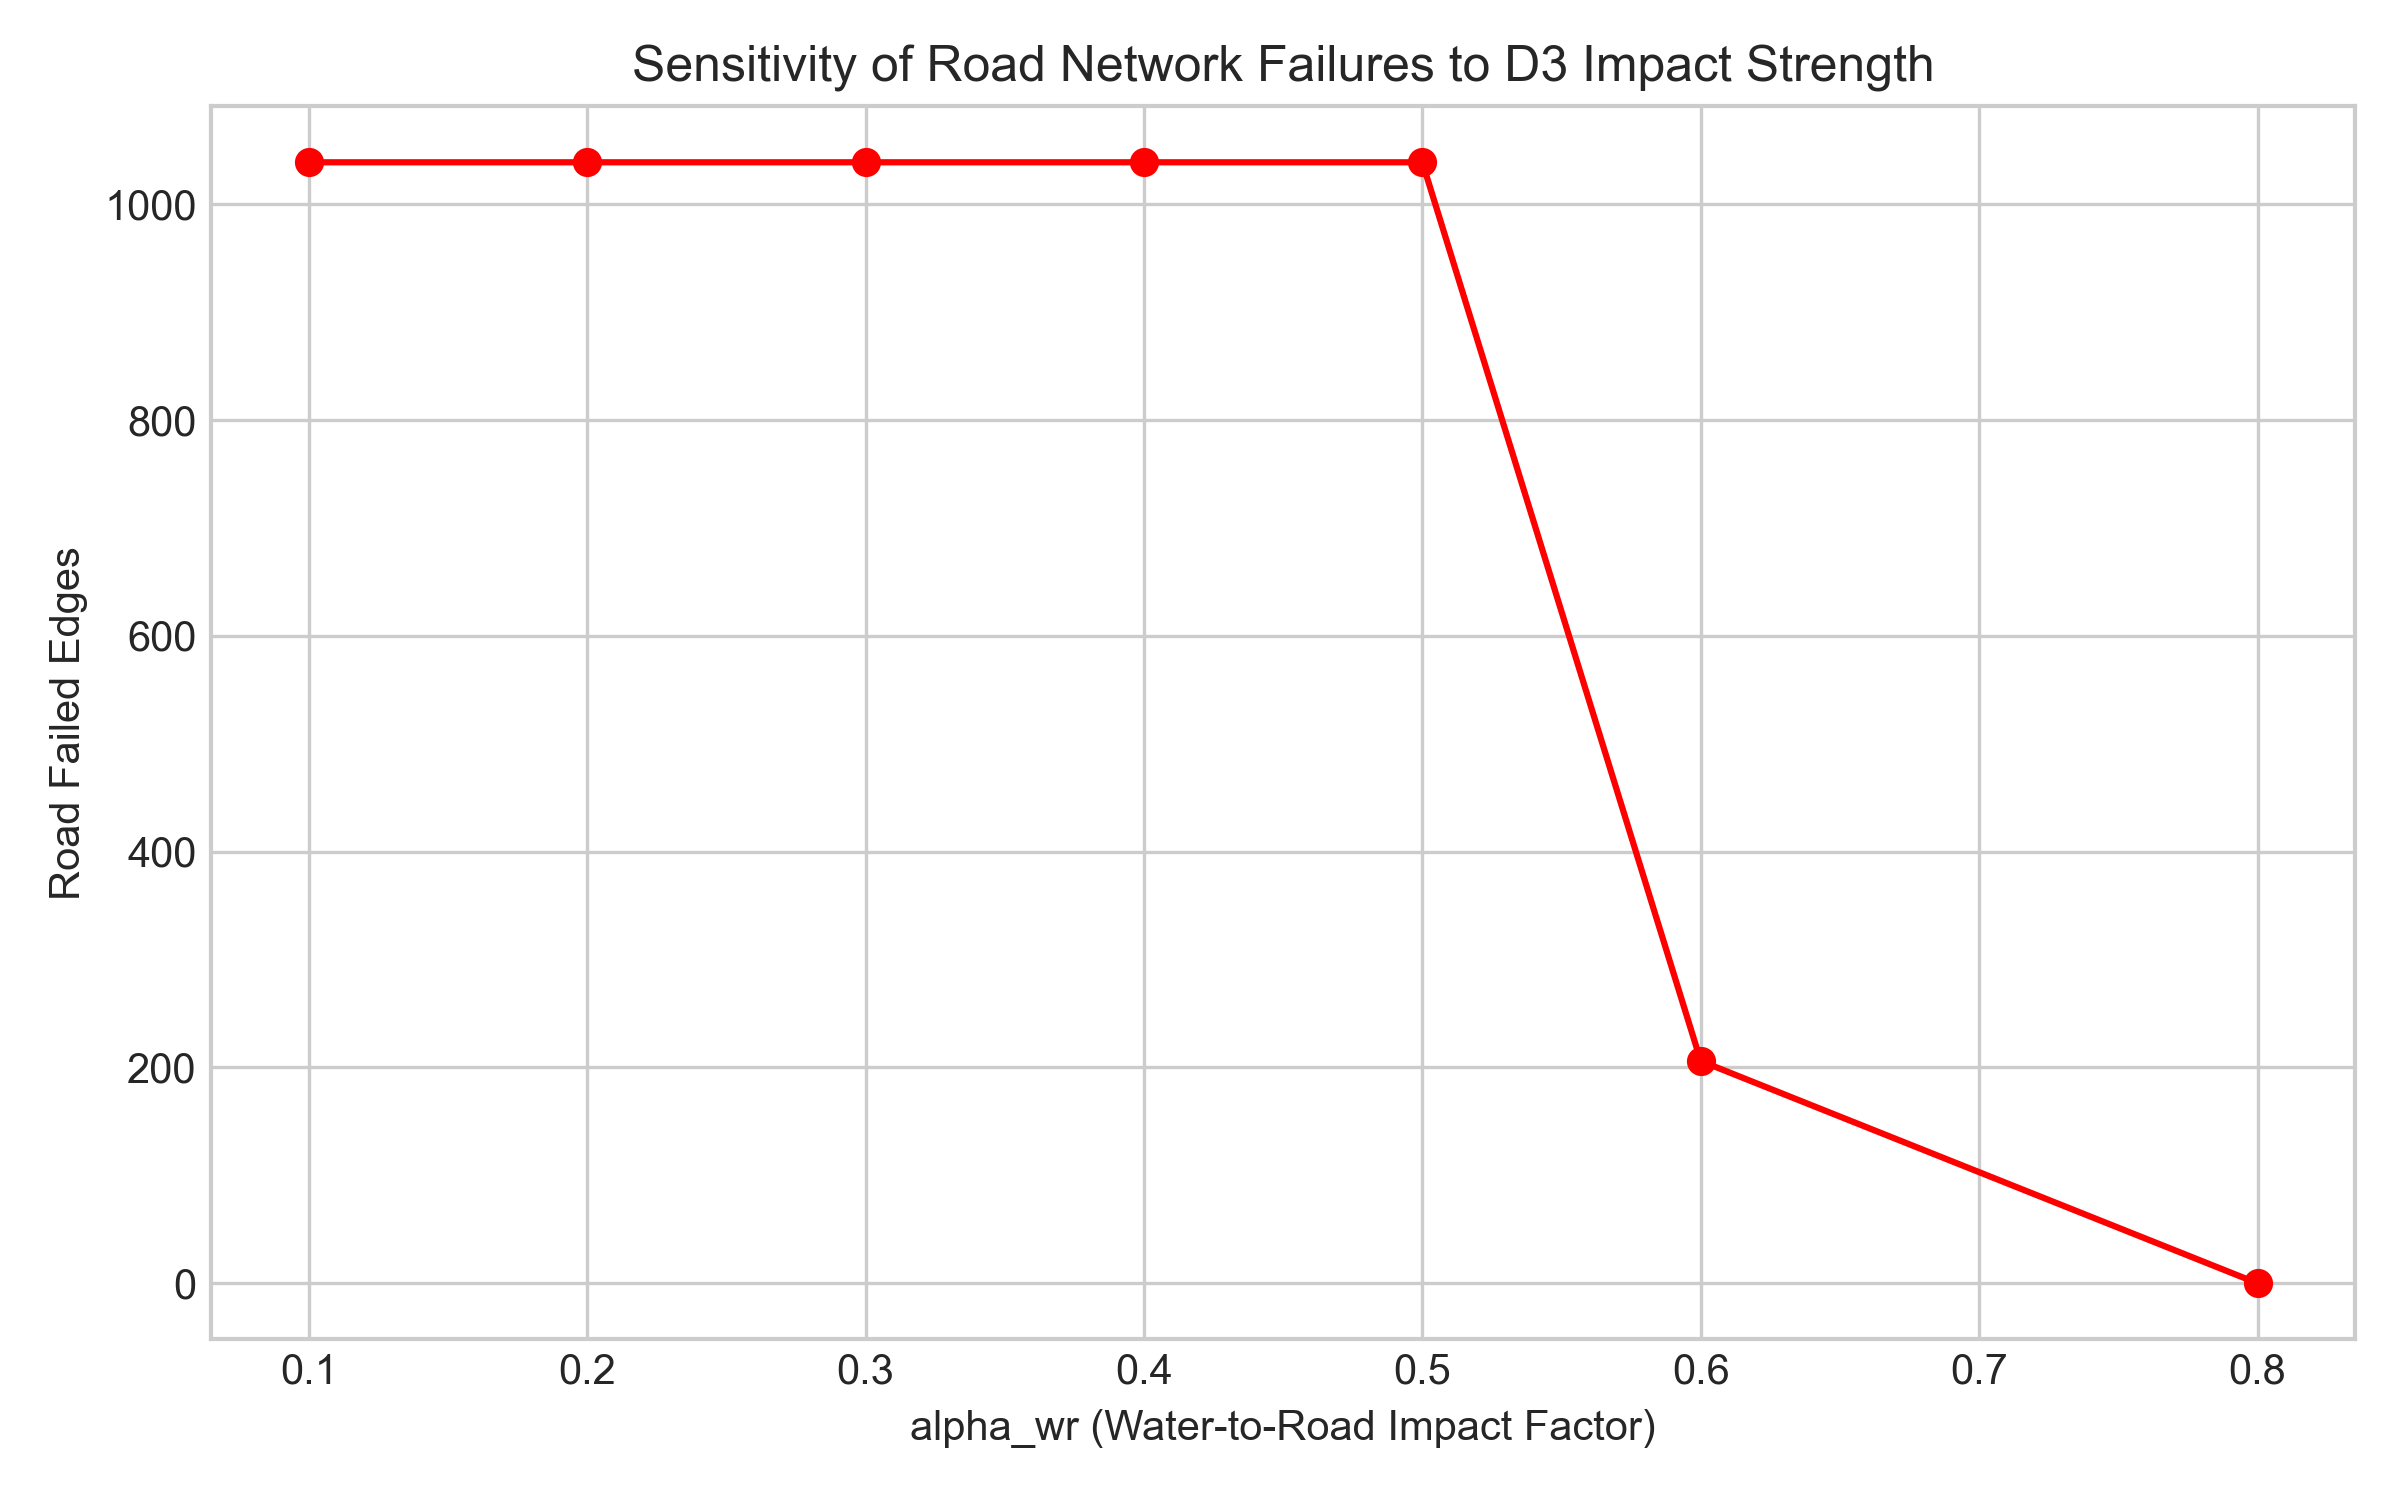
\includegraphics[width=\columnwidth]{sensitivity_alpha_wr_road_failures.png}
\caption{Parametric sensitivity of road edge failures to the water-induced lane capacity retention factor $\alpha_{wr} \in [0.10, 0.80]$, showing a sharp non-linear first-order tipping point at $\alpha_{wr} = 0.60$.}
\label{fig:sensitivity_alpha}
\end{figure}

\subsubsection{Water-to-Road Capacity Retention ($\alpha_{wr}$)}
The flood-induced capacity retention factor was swept across $\alpha_{wr} \in [0.10, 0.80]$ (Figure~\ref{fig:sensitivity_alpha}). The results reveal a sharp, non-linear phase transition at $\alpha_{wr} = 0.60$:
\begin{itemize}
    \item For $\alpha_{wr} \geq 0.70$, traffic diversion is accommodated smoothly by adjacent parallel arterials, yielding 0 secondary road failures.
    \item At $\alpha_{wr} = 0.60$, the system crosses a critical percolation threshold: localized bottleneck constriction triggers an immediate jump to 1,039 failed road edges.
\end{itemize}

\subsubsection{Power-to-Water Sensitivity ($s_{pw}$)}
Sweeping the electrical coupling parameter $s_{pw} \in [0.0, 1.0]$ indicated that while facility pumping throughput derates monotonically, downstream unmet demand is buffered by local network storage capacity, preventing catastrophic immediate pressure loss unless sustained over multiple operational hours.

%% ════════════════════════════════════════════════════════
\section{Operational Case Study: Central Silk Board 5 km Catchment}
\label{sec:case_study}

To evaluate the operational implications for urban emergency management, a high-resolution localized trial run was performed within a 5.0\,km geodesic radius centered on Central Silk Board Junction ($12.9172^\circ$\,N, $77.6228^\circ$\,E).

\subsection{Catchment Profile and Asset Inventory}

The 5\,km catchment spans Central Silk Board, HSR Layout, Koramangala, BTM Layout, Madiwala, and Bommanahalli. Using SciPy cKDTree geodesic queries, all critical utility assets within the radius were cataloged (Table~\ref{tab:asset_inventory}).

\begin{table}[!t]
\renewcommand{\arraystretch}{1.15}
\setlength{\tabcolsep}{3.0pt}
\caption{Critical Infrastructure Asset Inventory Within 5\,km of Central Silk Board Junction}
\label{tab:asset_inventory}
\centering
\resizebox{\columnwidth}{!}{%
\begin{tabular}{|l|l|c|c|}
\hline
\textbf{Asset ID} & \textbf{Facility Name / Description} & \textbf{Voltage / Cap.} & \textbf{Dist. (m)} \\
\hline
\hline
\multicolumn{4}{|l|}{\textit{KPTCL Electric Power Substations (9 Total):}} \\
SUB\_34 & St. John's Wood Substation        & 66/11\,kV  & 1,925 \\
SUB\_4  & Adugodi / Madiwala Substation     & 66/11\,kV  & 2,079 \\
SUB\_23 & Koramangala Bulk Hub Substation   & 220/66\,kV & 2,888 \\
SUB\_1  & HSR Layout Regional Bulk Hub      & 220/66\,kV & 3,274 \\
SUB\_43 & HSR Layout Distribution Substation& 66/11\,kV  & 3,274 \\
SUB\_6  & NIMHANS Healthcare Feeder         & 66/11\,kV  & 4,344 \\
SUB\_41 & NIMHANS Auxiliary Substation      & 66/11\,kV  & 4,344 \\
SUB\_9  & Golf Links Commercial Feeder      & 66/11\,kV  & 4,486 \\
SUB\_31 & Jayanagar Residential Substation  & 66/11\,kV  & 4,574 \\
\hline
\multicolumn{4}{|l|}{\textit{BWSSB Municipal Water Facilities (7 Total):}} \\
FAC\_47 & BTM Layout Ground Level Reservoir & 150 MLD    & 1,711 \\
FAC\_9  & Bommanahalli Booster Station      & 150 MLD    & 2,204 \\
FAC\_18 & HSR Layout Sector 1 Reservoir     & 150 MLD    & 2,667 \\
FAC\_45 & HSR Layout Sector 2 Pump House    & 150 MLD    & 3,389 \\
FAC\_11 & Dairy Circle / SG Palya Pump House& 150 MLD    & 4,288 \\
FAC\_1  & Ekaliki Water Supply Station      & 150 MLD    & 4,302 \\
FAC\_3  & Shudhi Water Works (Bellandur)    & 150 MLD    & 4,492 \\
\hline
\multicolumn{4}{|l|}{\textit{Roadway Transportation Network:}} \\
\multicolumn{4}{|l|}{3,752 intersection nodes and 4,299 directional links (100\% of CSB corridor).} \\
\hline
\end{tabular}%
}
\end{table}

\subsection{Localized Simulation Results and Contagion Mechanics}

The simultaneous triple-layer shock (SUB\_43 trip + trunk main rupture + intersection link closure) was injected at $t=0$. Table~\ref{tab:trial_results} compares the resulting contagion across coupling models.

\begin{table}[!t]
\renewcommand{\arraystretch}{1.2}
\setlength{\tabcolsep}{2.5pt}
\caption{Experimental Results of the 5\,km Central Silk Board Trial Run Across Coupling Models}
\label{tab:trial_results}
\centering
\resizebox{\columnwidth}{!}{%
\begin{tabular}{|l|c|c|c|c|}
\hline
\textbf{Model} & \textbf{Total Fails} & \textbf{Subs Failed (in 5km)} & \textbf{Road Fails (in 5km)} & \textbf{Delay} \\
\hline
\hline
M0 (Indep.)  & 6     & 1 / 9 (\textbf{11.1\%})  & 1     & 1.0002 \\
M1 (P $\rightarrow$ W) & 6   & 1 / 9 (\textbf{11.1\%})  & 1     & 1.0002 \\
M2 (P $\rightarrow$ R) & 6   & 1 / 9 (\textbf{11.1\%})  & 1     & 1.0002 \\
M3 (W $\rightarrow$ R) & 1,158 & 1 / 9 (\textbf{11.1\%}) & 1,153 & 1.0414 \\
\textbf{M7 (Full Triad)} & \textbf{1,608} & \textbf{9 / 9 (\textbf{100.0\%})} & \textbf{856} & \textbf{1.0371} \\
\hline
\end{tabular}%
}
\end{table}

\begin{figure}[!t]
\centering
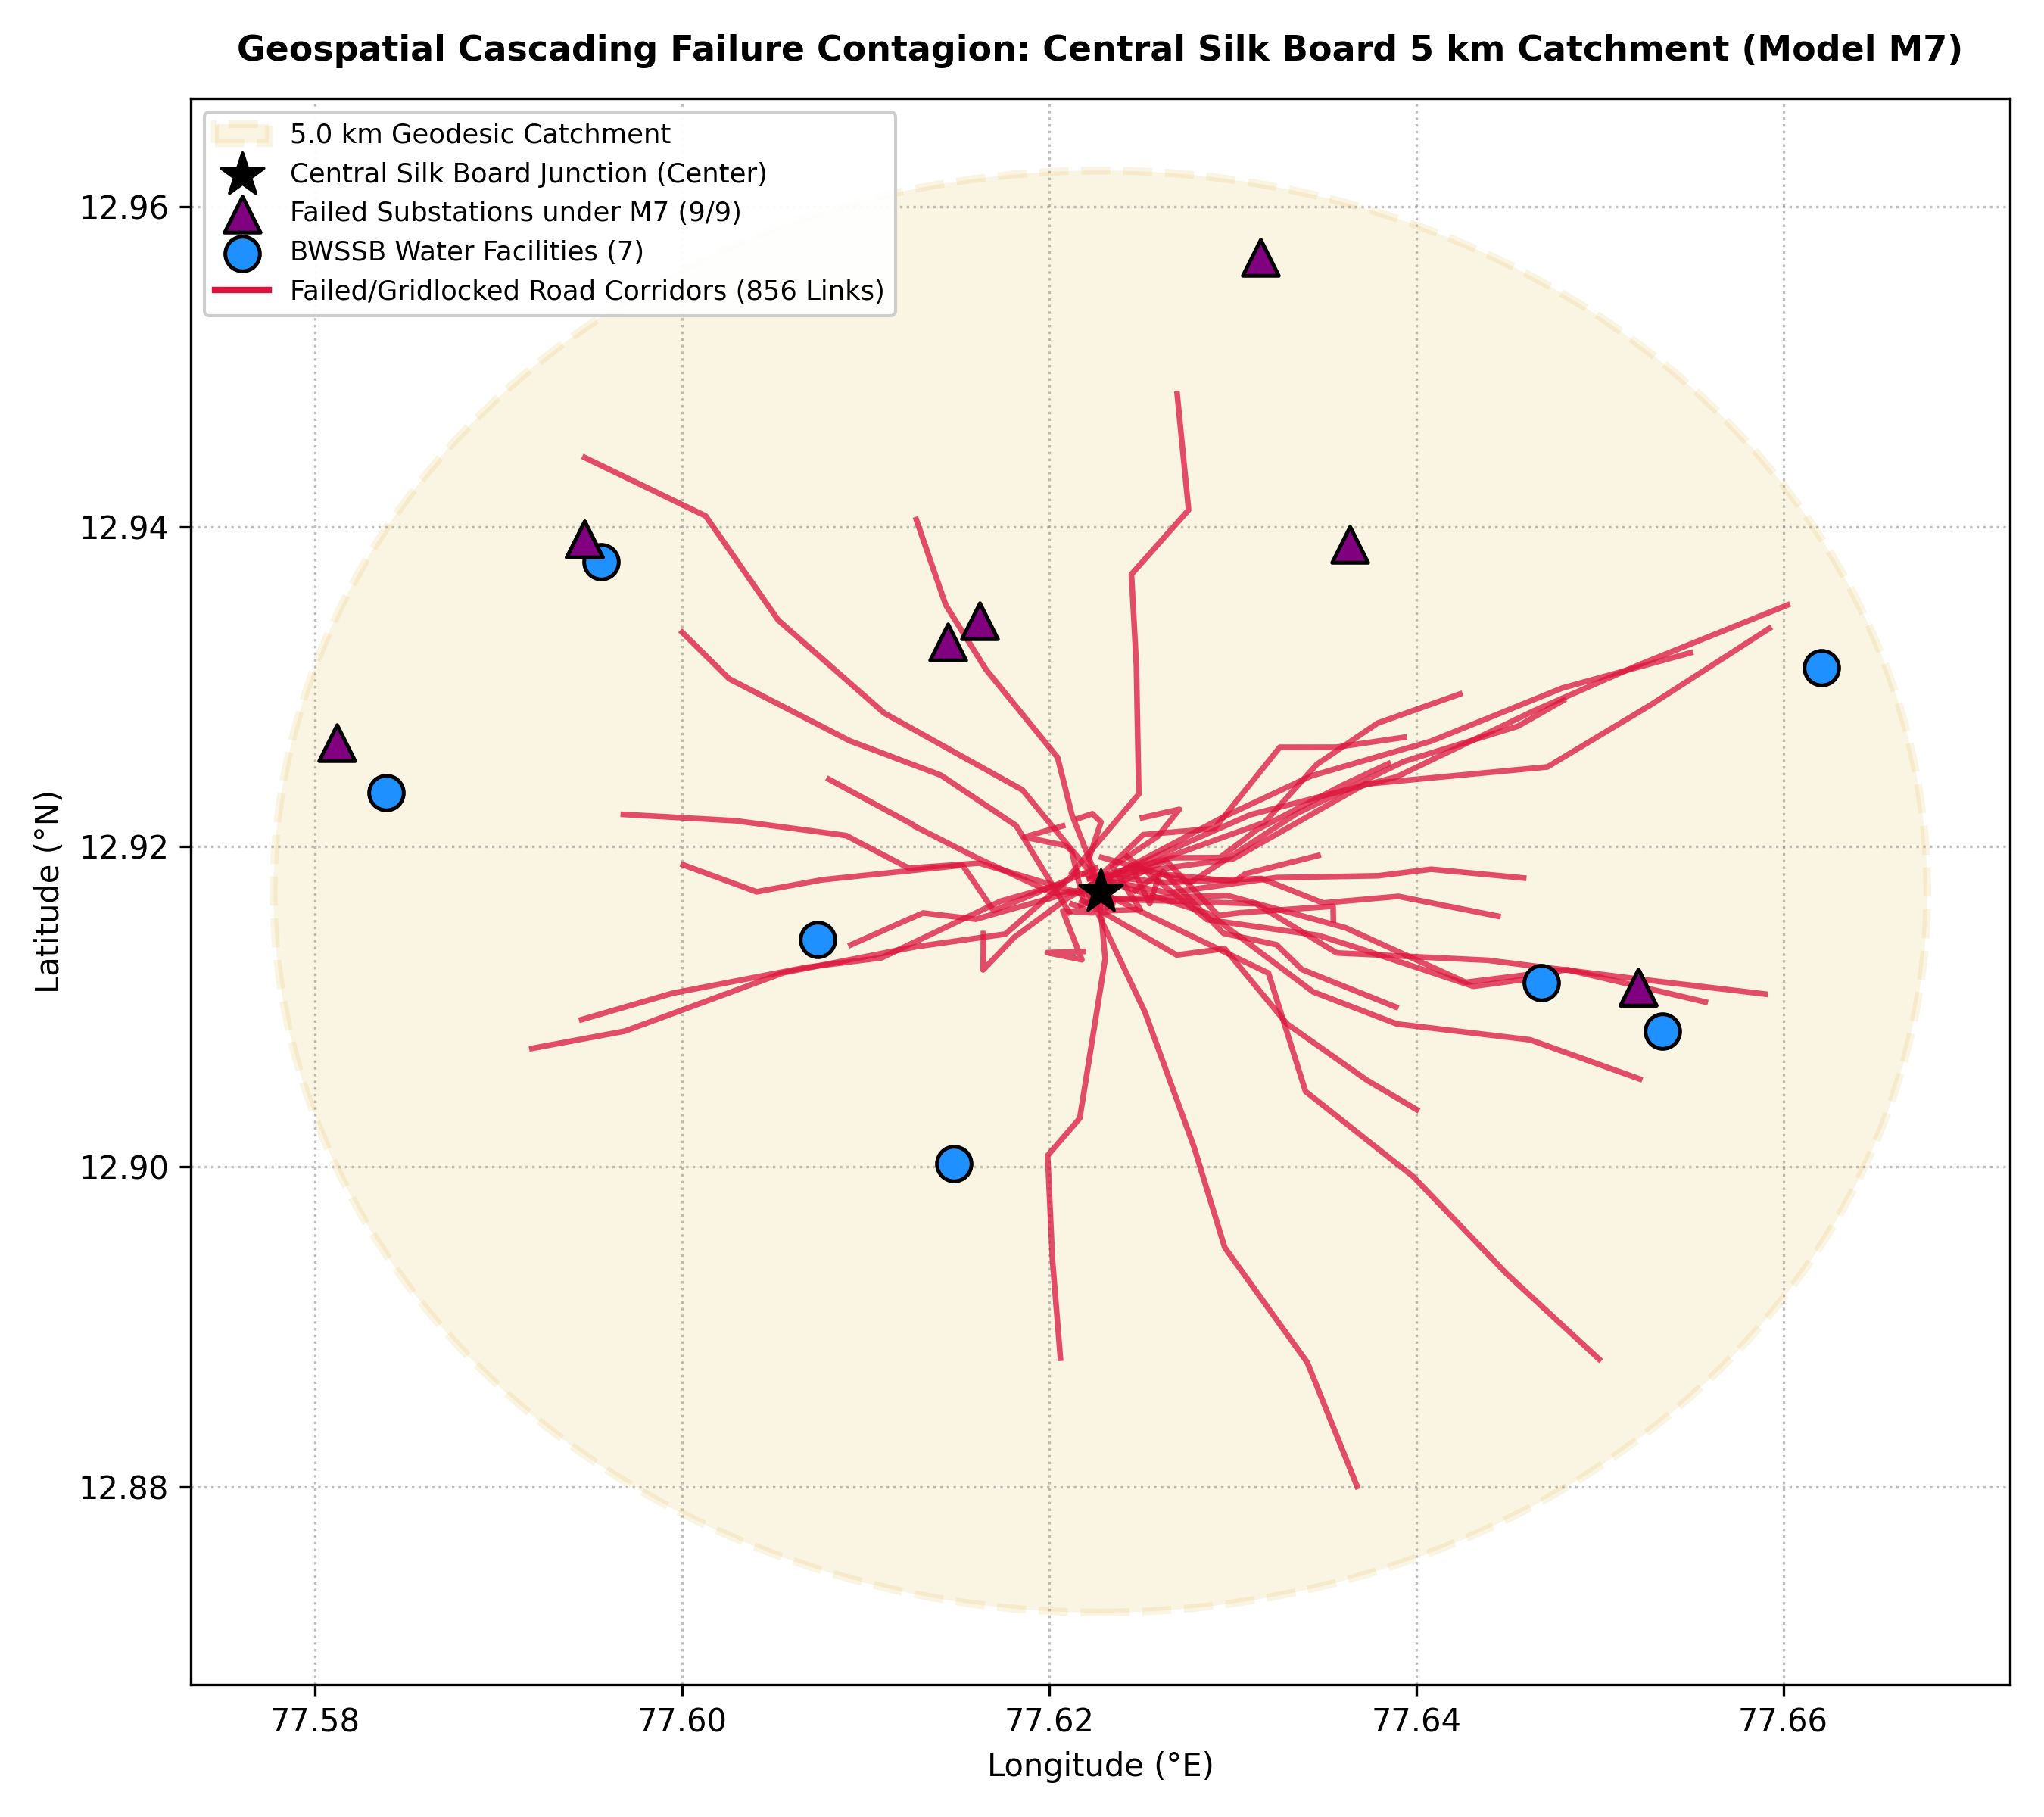
\includegraphics[width=\columnwidth]{trial_5km_silkboard_map.png}
\caption{Geospatial contagion map of the 5\,km Central Silk Board trial run (rendered using OpenStreetMap tiles). The golden circle demarcates the 5\,km boundary. Purple markers indicate the 9 regional power substations (all 9 failed under M7), blue markers denote the 7 BWSSB water facilities, and crimson segments show the 856 failed roadway links forming an impassable gridlock cordon.}
\label{fig:map_5km}
\end{figure}

The most critical operational insight is the substation contagion rate:
\begin{itemize}
    \item \textbf{Under Models M0 through M3:} Exactly 1 of 9 substations fails (11.1\%). The remaining 8 substations---including the major 220\,kV regional bulk transmission hubs SUB\_1 and SUB\_23, and the NIMHANS hospital healthcare feeder SUB\_6---remain operational. Traditional sectoral assessments would deem the regional electric power supply robust.
    \item \textbf{Under Model M7:} $\mathbf{100.0\%}$ of the regional substations fail ($\mathbf{9\text{ out of }9}$). Severe corridor congestion isolates substation sites from mobile maintenance and cooling logistics, driving them sequentially past their thermal failure limits.
\end{itemize}

Figure~\ref{fig:map_5km} depicts the geospatial distribution of this contagion within the 5\,km Silk Board catchment.

%% ════════════════════════════════════════════════════════
\section{Discussion and Policy Implications}
\label{sec:discussion}

\subsection{Breaking the ``Pairwise Trap'' in Urban Infrastructure Resilience}

For decades, urban resilience research and municipal contingency planning have operated under the assumption that pairwise coupling (e.g., studying electrical supply to water pumps or street flooding from water bursts) provides an adequate approximation of systemic multi-layer vulnerability. The empirical findings in Bengaluru fundamentally refute this assumption.

In Scenario S8, pairwise models predicted a maximum of 1,158 component failures, reporting a virtually undisturbed electric power grid. In contrast, full three-layer closed-loop modeling (M7) revealed 1,608 failures, including the complete collapse of 44 substations and 707 transmission lines. Pairwise models are structurally blind to these 747 power grid failures because they treat transportation networks as passive sinks rather than active, flow-dependent bottlenecks capable of reflecting destructive disruption back into the utility feeding networks.

\subsection{Municipal Infrastructure Hardening and Operational Playbook}

To mitigate cascading failure risks in co-located urban nexuses such as Central Silk Board, municipal agencies must transition from siloed management to coordinated, multi-utility defense:
\begin{enumerate}
    \item \textbf{Joint Utility Right-of-Way (ROW) Firewalls:} High-pressure municipal water transmission mains co-located beneath congested highway flyovers must be retrofitted with reinforced steel encasements and automated shut-off isolation valves to prevent roadway flooding from triggering corridor-wide traffic gridlock.
    \item \textbf{Emergency Utility Transit Priority Corridors:} Bangalore Traffic Police (BTP) and municipal disaster authorities must implement automated emergency priority corridors along the Outer Ring Road and Hosur Road to ensure dedicated travel lanes for BESCOM transformer cooling tankers and BWSSB repair vans during crisis events, preventing Feedback Channel D4 from tripping the electric grid.
    \item \textbf{Microgrid Islanding for Municipal Pumping Stations:} Major water booster installations (such as BTM Layout FAC\_47 and HSR Layout FAC\_18) should be equipped with solar-battery hybrid microgrids to maintain minimum head during 66\,kV feeder disruptions, preventing hydraulic water hammer surges from rupturing downstream pipelines.
    \item \textbf{Integrated Municipal SCADA Telemetry Exchange:} BESCOM, BWSSB, and BTP currently maintain isolated control centers. Real-time telemetry integration should automatically alert traffic signal controllers the moment a feeding substation exceeds 90\% load ratio, enabling proactive traffic diversion before complete blackout occurs.
\end{enumerate}

\subsection{Scientific Model Limitations and Threats to Validity}

To ensure methodological transparency, four model limitations should be acknowledged:
\begin{enumerate}
    \item \textbf{OpenStreetMap Disconnected Water Baseline:} Raw OpenStreetMap water distribution data in Bengaluru features 881 disconnected topological components, 828 of which lack an identified source facility. This produces an initial unserved demand of 16,814 MLD at $t=0$. Consequently, water disruption metrics must strictly be interpreted as deltas (relative changes from baseline) rather than absolute unserved quantities.
    \item \textbf{Quasi-Static Power Flow Proxy:} The power cascade model employs a headroom-weighted distance-decay load redistribution formulation based on apparent MVA ratings, rather than solving full AC Newton-Raphson load flow equations for voltage angles and reactive power deficits.
    \item \textbf{Topological Water Routing:} Water flow allocation utilizes shortest-path topological capacity constraints rather than dynamic non-linear Hazen-Williams or Darcy-Weisbach head loss equations in EPANET.
    \item \textbf{Uniform Initial Road Loading:} Due to the absence of publicly available, dynamic Origin-Destination (OD) travel matrices for Bengaluru, roadway links are initialized at a uniform baseline volume-to-capacity ratio of $V/C = 0.65$.
\end{enumerate}

%% ════════════════════════════════════════════════════════
\section{Conclusion}
\label{sec:conclusion}

This paper has presented an empirical, closed-loop, three-layer cascading failure framework for interdependent urban utility networks, grounded in metropolitan geospatial datasets from Bengaluru, India. By formulating continuous proportional degradation functions, hydraulic water-hammer shock approximations, BPR volume-delay traffic redistribution, and three closed-loop cyclic feedback mechanisms (Road $\rightarrow$ Power, Road $\rightarrow$ Water, and Water $\rightarrow$ Road), the framework overcomes the structural limitations of conventional binary and pairwise models.

Across an 8-level coupling hierarchy (M0--M7) evaluated on 8 disruption scenarios (S1--S8), the results demonstrate a substantial Higher-Order Interaction Gain ($G = +450$ component failures in Scenario S8), representing a 38.86\% increase in systemic disruption over the strongest pairwise model. In a localized 5.0\,km case study around Central Silk Board Junction, traffic gridlock induced by a water pipe rupture choked substation maintenance and cooling logistics, triggering a 100\% failure contagion across all 9 regional substations (compared with only 11.1\% predicted under independent and pairwise models). These findings demonstrate that evaluating infrastructure networks in isolation or through pairwise approximations severely underestimates systemic vulnerability, providing an urgent operational mandate for integrated, multi-agency urban resilience planning.

\begin{thebibliography}{00}
\bibitem{b1}
Y. Tang, J. Piao, H. Wang, S. Rajib, and Y. Li,
``Predicting Cascade Failures in Interdependent Urban Infrastructure Networks,''
arXiv preprint arXiv:2503.02890, 2025.

\bibitem{b2}
Wu et al.,
``Vulnerability Analysis of Interdependent Infrastructures Considering the Sensitivity of Components to Different Risks,''
2023.

\bibitem{b3}
L. Lu et al.,
``Vulnerability of Interdependent Urban Infrastructure Networks: Equilibrium after Failure Propagation and Cascading Impacts,''
\textit{Computer-Aided Civil and Infrastructure Engineering},
vol. 33, no. 4, pp. 300--315, 2018.

\bibitem{b4}
Rahimi-Golkhandan et al.,
``Predictive Resilience of Interdependent Water and Transportation Infrastructures: A Sociotechnical Approach,''
2022.

\bibitem{b5}
Y. Zhao et al.,
``Failure Dependence and Cascading Failures: A Literature Review and Research Opportunities,''
\textit{Reliability Engineering \& System Safety},
vol. 256, Art. no. 110766, 2025.

\bibitem{b6}
W. Liu et al.,
``Resilience Assessment of Urban Connected Infrastructure Networks,''
\textit{Scientific Reports},
vol. 15, Art. no. 19770, 2025.

\bibitem{b7}
H. Jia, F. Li, L. Yang, Q. Luo, and Y. Li, ``Dynamic cascading failure analysis in congested urban road networks with self-organization,'' \emph{IEEE Access}, vol. 8, pp. 17916--17925, 2020, doi: 10.1109/ACCESS.2020.2968048.

\bibitem{b8}
J. Sun and Q. J. Xiang, ``Identification of critical links based on the failure consequence evaluation,'' in \emph{Proc. 3rd IEEE Int. Conf. Intell. Transp. Eng. (ICITE)}, Singapore, 2018, pp. 318--323, doi: 10.1109/ICITE.2018.8492704.

\bibitem{b9}
W. Liu, Y. Zhao, H. Miao, Y. Zhang, Z. Liu, and L. Zhang, ``Identification of power information network system vulnerabilities by using cascading failure analysis and differential evaluation with maturity factor,'' in \emph{Proc. Int. Conf. Integr. Intell. Commun. Syst. (ICIICS)}, Kalaburagi, India, 2024, pp. 1--5, doi: 10.1109/ICIICS63763.2024.10859930.

\bibitem{b10}
Q. Shi, Y. Yan, W. Liu, B. Zeng, Z. Wang, and F. Li, ``Resilience assessment of urban power network considering multi-stage electrical-water fault propagation,'' \emph{IEEE Trans. Power Syst.}, vol. 40, no. 4, pp. 2819--2831, Jul. 2025, doi: 10.1109/TPWRS.2024.3420114.

\bibitem{b11}
S. R., ``Blore infrastructure failure cascade detection,'' GitHub repository. [Online]. Available: \url{https://github.com/Spoorthi227/blore-infra-failure-cascade-detection}.

\bibitem{b12}
Overpass Turbo, ``A web-based data mining tool for OpenStreetMap using the Overpass API.'' [Online]. Available: \url{https://overpass-turbo.eu/}.

\bibitem{b13}
Open Infrastructure Map, ``Open map of the world's infrastructure based on OpenStreetMap data.'' [Online]. Available: \url{https://openinframap.org/}.

\bibitem{b14}
J. Y. Yen, ``Finding the K shortest loopless paths in a network,'' \emph{Manage. Sci.}, vol. 17, no. 11, pp. 712--716, Jul. 1971.

\bibitem{b15}
\emph{Traffic Assignment Manual}, U.S. Bureau of Public Roads, U.S. Dept. Commerce, Washington, DC, USA, 1964.

\bibitem{b16}
P. K. Huynh, C. Hoang, D. Nguyen, T. Truong, and T. T. Q. Le, ``Multi-scale system reliability analysis of multi-layer network infrastructures,'' in \emph{Proc. Annu. Rel. Maintainability Symp. (RAMS)}, Destin, FL, USA, 2025, pp. 1--7, doi: 10.1109/RAMS48127.2025.10935270.

\bibitem{b17}
S. Kumar, S. Vaishya, S. S. Rani, P. Agarwal, D. Chandra, and R. S. Tomar, ``Multi-hazard resilient infrastructure modeling using digital twin technology combined with predictive analytics in modern smart city frameworks,'' in \emph{Proc. IEEE Int. Conf. Recent Trends Comput. Smart Mobility (RCSM)}, Bhopal, India, 2025, pp. 1--6, doi: 10.1109/RCSM67767.2025.11506702.

\bibitem{b18}
C. Ma, K. Sun, W. Li, Z. Lu, C. Wei, and K. Wen, ``Automated repair, topological reconstruction, and attribute enhancement of AI-derived fragmented road networks,'' in \emph{Proc. 15th Int. Conf. Power Energy Syst. (ICPES)}, Chongqing, China, 2025, pp. 582--586, doi: 10.1109/ICPES68632.2025.11371879.

\bibitem{b19}
X. Zhang, W. Qin, X. Jing, J. Liu, X. Han, and P. Wang, ``Power system resilience assessment considering the occurrence of cascading failures,'' in \emph{Proc. Int. Conf. Power Syst. Technol. (PowerCon)}, Jinan, China, 2023, pp. 1--5, doi: 10.1109/PowerCon58120.2023.10331511.

\bibitem{b20}
H. Wan, W. Liu, Q. Shi, R. Zhu, X. Zhang, and J. Zhao, ``Real-time service restoration of coupled power-water systems considering the spatio-temporal cascading failure,'' \emph{IEEE Trans. Smart Grid}, vol. 17, no. 1, pp. 178--192, Jan. 2026, doi: 10.1109/TSG.2025.3602929.

\end{thebibliography}

\begin{IEEEbiographynophoto}{Dr. Manonmani S} is currently working as an Associate Professor at the Department of Computer Science and Engineering, RV College of Engineering, Bengaluru, Karnataka, India. Her research interests include data science, machine learning, deep learning, image processing, web technologies, and prompt engineering. She has over 16 years of teaching experience and has led several industry-sponsored research and consultancy projects.
\end{IEEEbiographynophoto}
\begin{IEEEbiographynophoto}{Spoorthi Ravi Pratap} is currently pursuing the B.E. degree in Computer Science and Engineering at RV College of Engineering, Bengaluru, Karnataka, India. She is currently in the sixth semester of her undergraduate studies.
\end{IEEEbiographynophoto}
\begin{IEEEbiographynophoto}{Siya Pranesh Kurandwad} is currently pursuing the B.E. degree in Computer Science and Engineering at RV College of Engineering, Bengaluru, Karnataka, India. She is currently in the sixth semester of her undergraduate studies.
\end{IEEEbiographynophoto}
\begin{IEEEbiographynophoto}{Poornashree H. V.} is currently pursuing the B.E. degree in Information Science and Engineering at RV College of Engineering, Bengaluru, Karnataka, India. She is currently in the sixth semester of her undergraduate studies.
\end{IEEEbiographynophoto}
\begin{IEEEbiographynophoto}{Neha T. N.} is currently pursuing the B.E. degree in Computer Science and Engineering (Cyber Security) at RV College of Engineering, Bengaluru, Karnataka, India. She is currently in the sixth semester of her undergraduate studies.
\end{IEEEbiographynophoto}
\EOD

\end{document}

